\chapter[Results]{Results}
\label{cha:Results}

This chapter, shows the results that could be obtained using, the experiments, mentioned in chapter \ref{cha:Experiment}. Those results contain either numbers, for assessing the model performance with a certain error performance, but also of graphics, displaying the outputs of the models. The outputs of the models, being spectrograms, will get compared with their corresponding input spectrograms. Also as the encoded features that get output of the encoder, get assessed, those get displayed as well. 


\section{Results of initial Experiments}
Despite the initial experiments, are just based on a prove of concept implementation, without real synthesis, those results are also regarded as important. Not at least as they are part of the development during the research. 


<Signal plots comparison>
<Frames comparison>
<spectrograms input output comparison

\section{Results regarding models with single Frequency Vectors}
As described in chapter \ref{cha:Experiment} experiments have been conducted by using the single frequency vectors of the spectrograms. As a model, a 18 layer deep neural network with 1D convolutions has been trained on the reconstruction of single frequency vectors. 
Throughout the development different settings have been tried out in order to find a model with an optimal training process and performance. The amount of data on which the model has been trained on, has been varied as different performances regarding the convergence could be observed. First trainings have been made on keyboard\_synthetic mixed with guitar\_acoustic. Here it could be observed, that no sufficient convergence could be reached (MSE > 200). Training a distinct model per instrument source, showed that the instrument source has a significant influence on the convergence. For example a model trained solely trained on keyboard\_synthetic converged better then a model with guitar\_acoustic. Comparing the performance of a network trained on guitar\_acoustic with one trained on e.g. guitar\_electronic, showed that with the latter a better score could be reached (\textasciitilde 17). Therefore the decision was made, to combine keyboard\_synthetic and guitar\_electronic instead of acoustic, for the training. Compared to the one mixed with guitar\_acoustic a score of \textasciitilde 78 could be reached. Subsequently more instrument sources got added, until the whole training dataset was utilized. This model showed the best performance and was chosen to be considered for the ongoing experiments. The next table \ref{tab:res_scores_1Dcae} shows the error scores of this model. As a short note, each trained model was chosen based on the best validation error score. 

\begin{table}[htb!]
    \centering
    \begin{tabular}{|c|c|}
        \hline
         & \textbf{MSE-Score} \\
         \hline
        \textbf{Training} & 4,237 \\
        \hline
        \textbf{Validation} & 4,638 \\
        \hline
        \textbf{Test} & 1,190 \\
        \hline
    \end{tabular}
    \caption{MSE-Scores 1D convolutional autoencoder (8 epochs)}
    \label{tab:res_scores_1Dcae}
\end{table}

Here it can be seen that the error scores for training and validation are rather close, while the score on the held out test set was significantly smaller. This score could be reached with a training over 8 epochs and was considered as the best score, as after those 8 epochs the validation score increased again (despite decreasing training score). The next graphic \ref{tab:res_scores_1D_pitch} is also interesting as it shows, the error scores on the test set, regarding different pitches. In this case it can be seen, that the numbers does not really have a significant variance.

\begin{table}[htb!]
    \centering
    \begin{tabular}{|c|c|}
        \hline
         \textbf{Pitch} & \textbf{MSE-Score} \\
         \hline
         \textbf{030} & 1,049\\
         \hline
         \textbf{035} & 1,393\\
         \hline
         \textbf{040} & 0,935\\
         \hline
         \textbf{045} & 1,096\\
         \hline
         \textbf{050} & 1,019\\
         \hline
         \textbf{055} & 1,108\\
         \hline
         \textbf{060} & 1,086\\
         \hline
         \textbf{065} & 1,111\\
         \hline
         \textbf{070} & 1,164\\
         \hline
         \textbf{075} & 1,041\\
         \hline
         \textbf{080} & 1,177\\
         \hline
         \textbf{085} & 1,753\\
         \hline
         \textbf{090} & 1,100\\
         \hline
         \textbf{095} & 1,796\\
         \hline
         \textbf{100} & 2,043\\
         \hline
    \end{tabular}
    \caption{MSE-Scores for specific pitch classes using 1D convolutional autoencoder.}
    \label{tab:res_scores_1D_pitch}
\end{table}

\subsection{Experiments of single reconstruction}
Having the trained network, this one got evaluated towards the ability of reconstructing audio spectrograms and further on recreating the sounds. The next graphics (\ref{fig:res_1D_input_output}, \ref{fig:res_1D_emb} and \ref{fig:res_1D_input_output_sig}) show the result of taking a guitar sample as input and reconstructing it. 

\begin{figure}[htb!]
    \centering
    \makebox[\textwidth][c]{\begin{tabular}{@{}cc@{}}
        \makebox{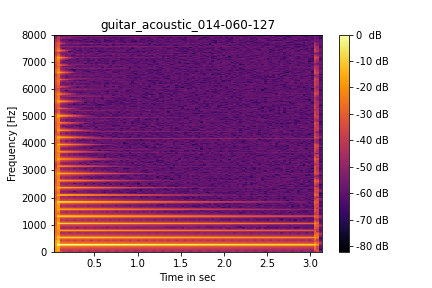
\includegraphics[width=0.5\textwidth]{images/approach/guitar_acoustic_014-060-127.png}}&
        \makebox{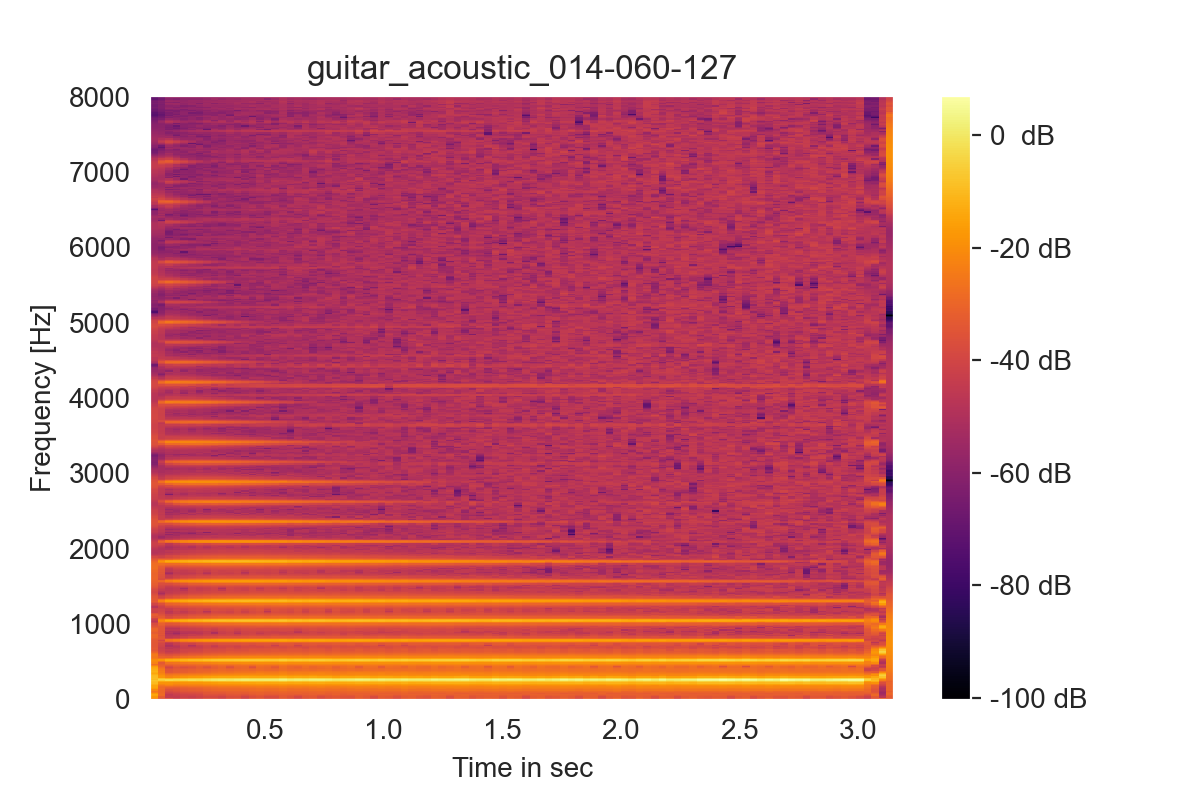
\includegraphics[width=0.5\textwidth]{images/results/rec_guitar_acoustic_014-060-127.png}}\\
        (a) & (b)
    \end{tabular}}
    \caption{input spectrogram ~(a), reconstructed spectrogram. ~(b).}
    \label{fig:res_1D_input_output}
\end{figure}

With a special look onto the reconstructability of spectrograms, figure \ref{fig:res_1D_input_output} shows the input spectrogram and the generated output spectrograms from the network. Here it can be seen, that the reconstructed spectrogram, differs in a few points from the input spectrogram. First of all it can be seen, that across the frequency areas with little energy in the input spectrogram, in the output more energy is present. This also means that between those areas and the sound-characteristic high energy areas, less difference is present. Furthermore regarding the original broad spectra at the beginning and at the end, are hardly present in the output spectrogram. Knowing that these represent the stroke and the damp of the string, it can be said, that these are not present in the output. This gets also confirmed through looking at the time-domain signal but moreover on listening to the final sound. 

\begin{figure}[htb!]
    \centering
    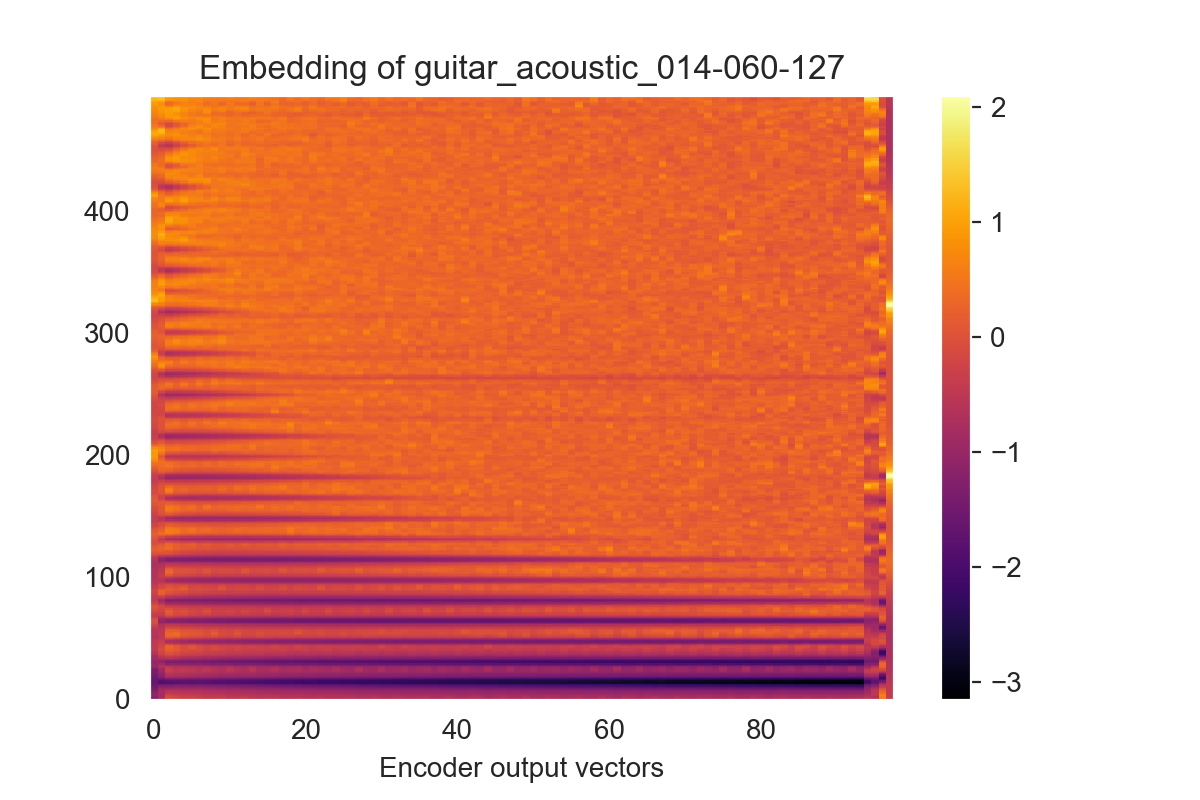
\includegraphics[width=0.5\textwidth]{images/results/emb_guitar_acoustic_014-060-127.png}
    \caption{Encoding of guitar acoustic.}
    \label{fig:res_1D_emb}
\end{figure}

Looking at the graphic that depicts the embedded space, there it already can be seen that those broad spectra are not preserved. A final look onto the time domain plots also reveal, that there's no impulse at the beginning of the signal. Furthermore it also can be said, that the amplitude in general differs in its course but also in how strong it is.

\begin{figure}[htb!]
    \centering
    \makebox[\textwidth][c]{\begin{tabular}{@{}cc@{}}
        \makebox{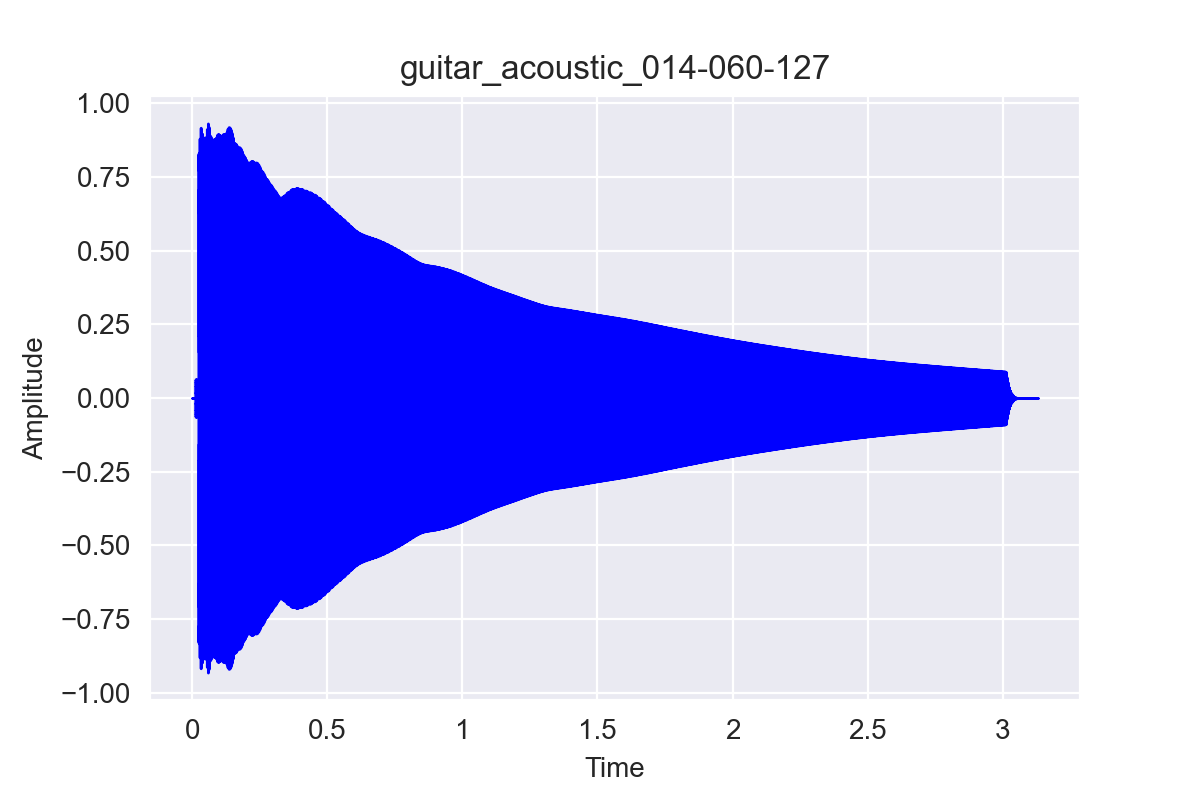
\includegraphics[width=0.5\textwidth]{images/results/inp_guitar_acoustic_014-060-127.png}}&
        \makebox{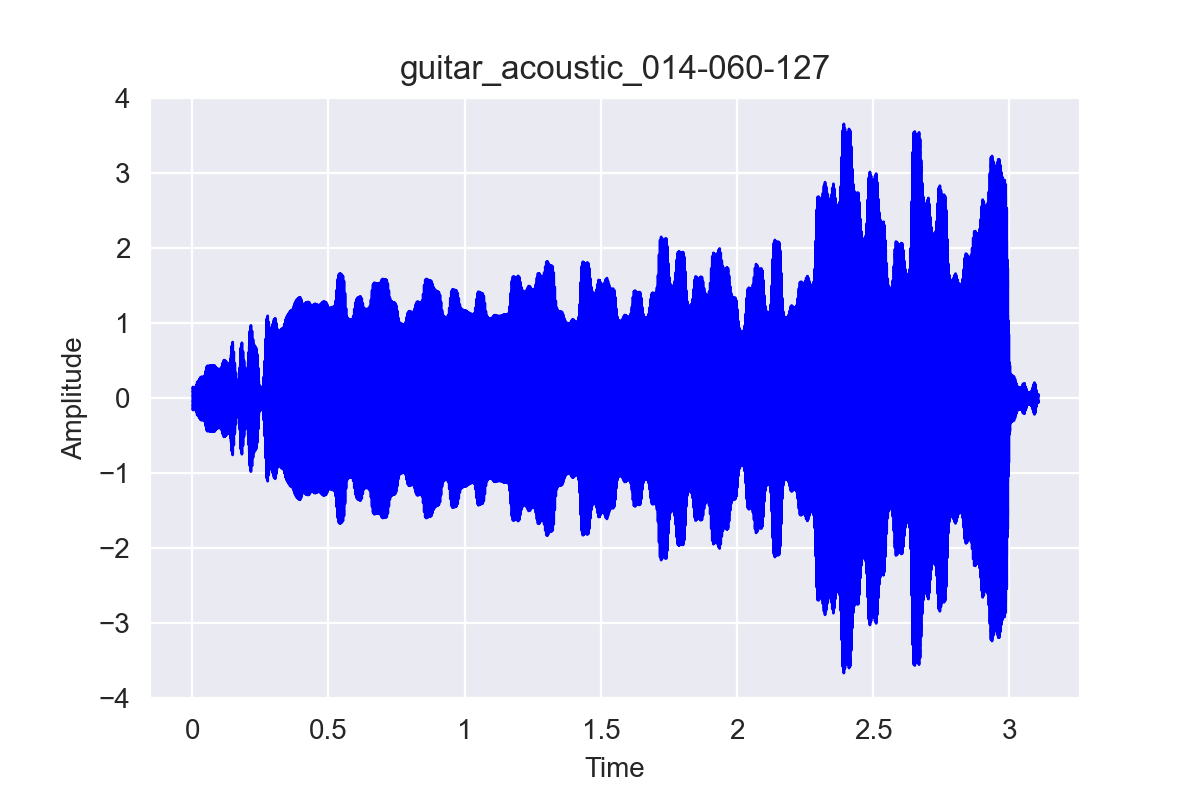
\includegraphics[width=0.5\textwidth]{images/results/out_guitar_acoustic_014-060-127.png}}\\
        (a) & (b)
    \end{tabular}}
    \caption{input signal ~(a), output signal ~(b).}
    \label{fig:res_1D_input_output_sig}
\end{figure}


\subsection{Experiments with interpolation in embedding}
With this kind of 1D convolutional autoencoder first experiments were made, that use interpolation in embedded space to synthesize novel sounds. In chapter \ref{cha:Approach} and \ref{cha:Experiment} the concept has already been described in detail. Having this concept, instrument sources were chosen, which in order got encoded and interpolated together to in order form a new embedding. The next graphic \ref{fig:res_1D_input_interpolation} shows two input instruments that were chosen to create a novel sound. For this representation an acoustic guitar and acoustic brass sample were taken and encoded.

\begin{figure}[htb!]
    \centering
    \makebox[\textwidth][c]{\begin{tabular}{@{}cc@{}}
        \makebox{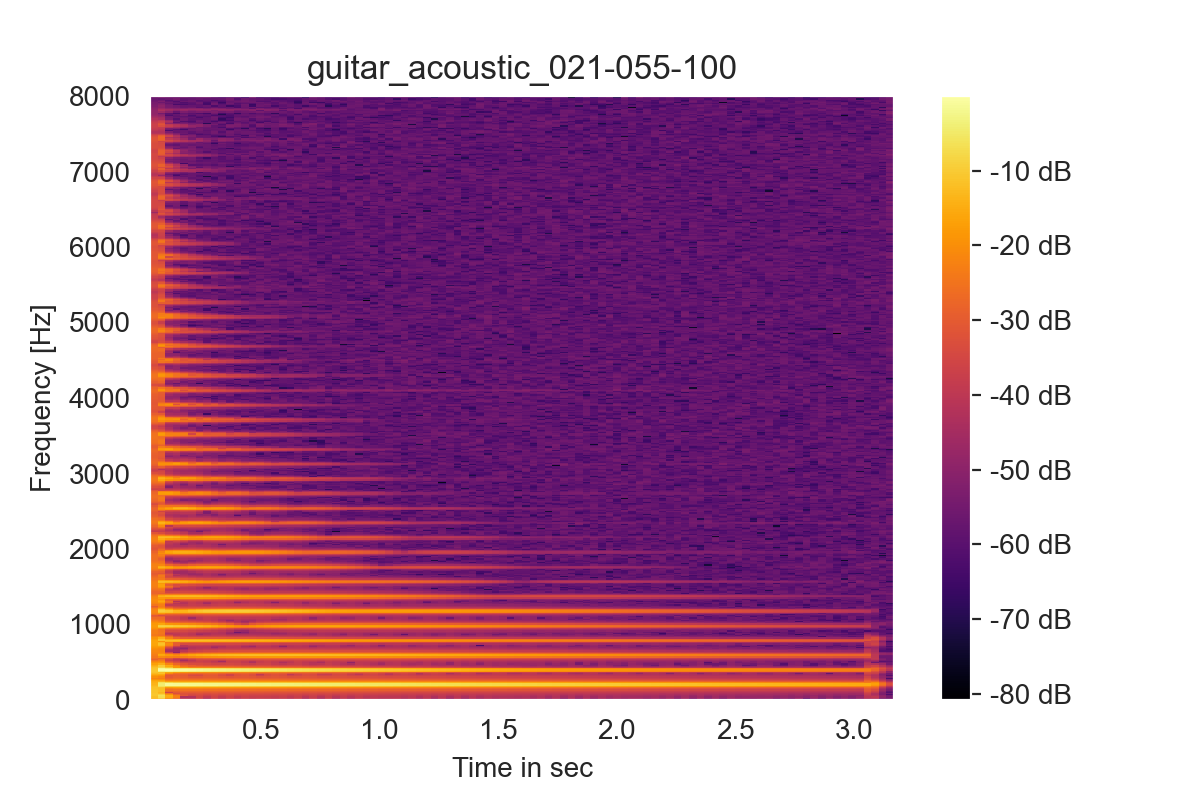
\includegraphics[width=0.55\textwidth]{images/results/guitar_acoustic_021-055-100.png}}&
        \makebox{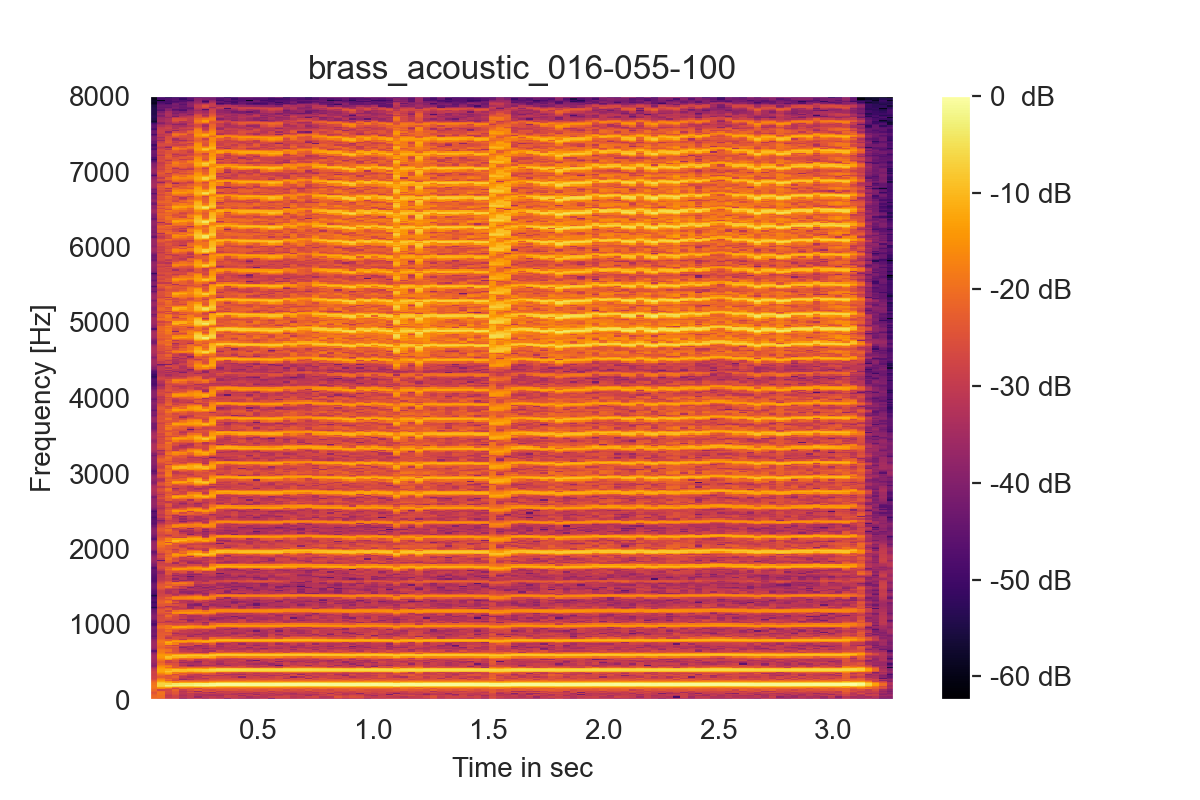
\includegraphics[width=0.55\textwidth]{images/results/brass_acoustic_016-055-100.png}}\\
        (a) & (b)
    \end{tabular}}
    \caption{guitar acoustic ~(a), brass acoustic ~(b).}
    \label{fig:res_1D_input_interpolation}
\end{figure}

After encoding, the outputs were taken and interpolated as can be seen in the next figure \ref{fig:res_1D_interpolation}a. As it can be seen, those embeddings are a compressed form of the input spectrograms. When looking onto the generated interpolated embedding, it can be said, that this one incorporates both instruments encoded features. Having this new vector, this one was fed into the decoder network to in order generate an output spectrogram that can be seen in figure \ref{fig:res_1D_interpolation}b. 

\begin{figure}[htb!]
    \centering
    \makebox[\textwidth][c]{\begin{tabular}{@{}cc@{}}
        \makebox{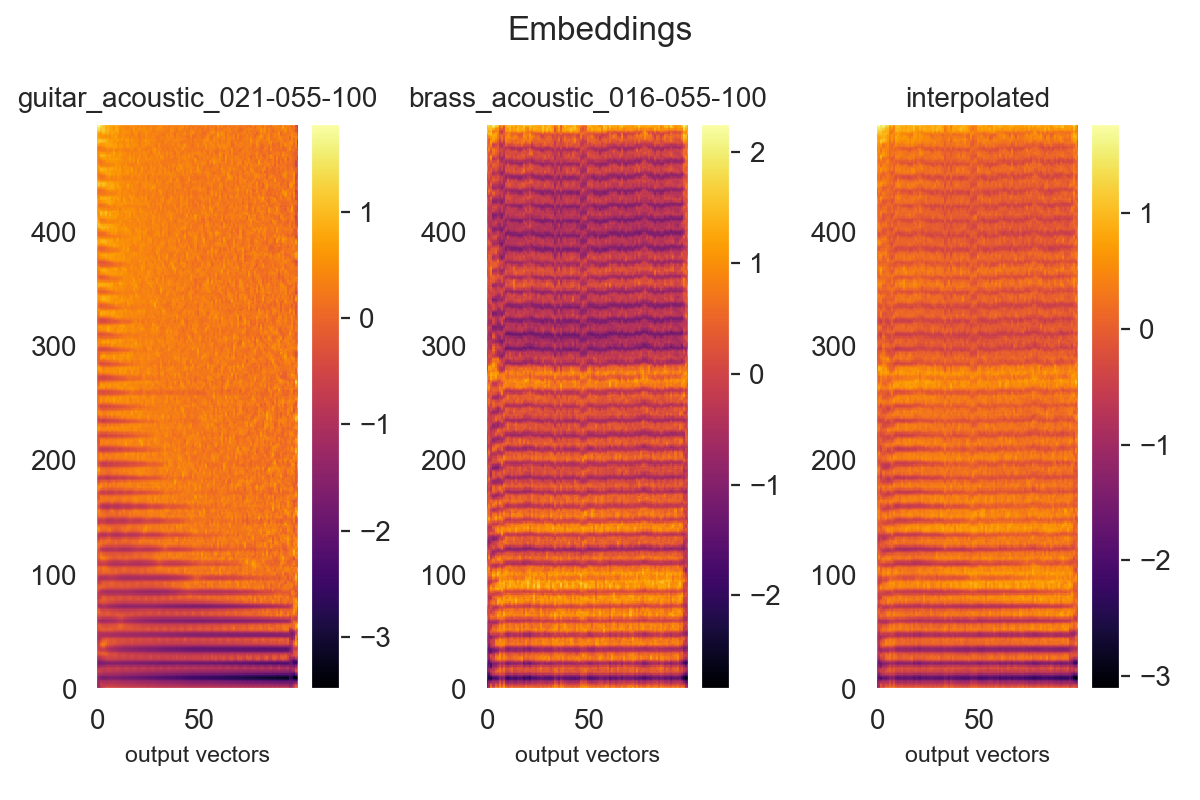
\includegraphics[width=0.55\textwidth]{images/results/interp_emb_guitar_acoustic_021-055-100&brass_acoustic_016-055-100.png}}&
        \makebox{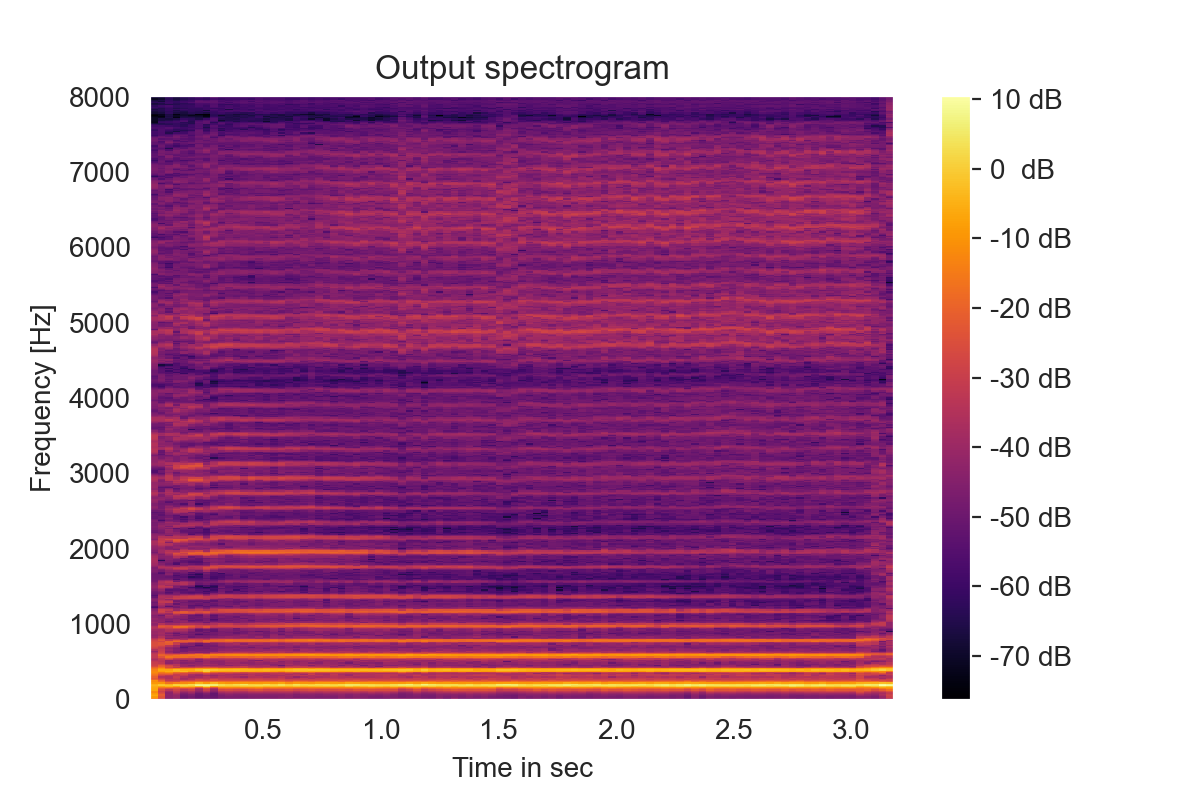
\includegraphics[width=0.55\textwidth]{images/results/guitar_acoustic_021-055-100&brass_acoustic_016-055-100_output_spec.png}}\\
        (a) & (b)
    \end{tabular}}
    \caption{embedding interpolation ~(a), output signal ~(b).}
    \label{fig:res_1D_interpolation}
\end{figure}

Having the final spectrogram here as output, it can be seen, that spectral data of both input spectrograms are basicaly contained. Similar to the output spectrogram in figure \ref{fig:res_1D_input_output}b this one also does not contain the impulse (guitar stroke) at the beginning. To finally obtain a listenable sound, the output spectrogram has to get converted back to time-domain, which in this case gets done with the Griffin-Lim algorithm \cite{Griffin1984} as no phase information is present. By listening to the final obtained sample, it can be heard, that it already contains features of both instruments despite the guitar is not as present as expected (guitar stroke not audible). Furthermore the sound contains distortion which is not desirable.

To improve the quality of the output but also to examine the performance of other types of networks some further experiments have been made using 2D convolutions but also additional post-processing steps.

\section{Results of experiments with spectrogram frames}
The here shown results, correspond to the described experiments in section \ref{sec:exp_spec_slice}. Here again a 2D convolutional autoencoder has been utilized to (re)synthesize audio. As input data for the neural networks, overlapping spectrograms snippets with the length of 3 along the time axis have been considered. In contrast to the previous network, this was supposed to bring better results, regarding the output but especially to preserve transients. As different networks with different stridings (compression) were trained and used, the results should also show the differences in the output but also in their quality regarding audio (re)synthesis. Additionally the encoded data gets examined by calculating the correlation coefficients between samples (mostly of the same pitch). By that it can be seen how much the encodings of different instruments differ. Additionally it also can be examined how good the different networks extract the essential features of the input data. Throughout the project these correlation coefficients got depicted in a so-called correlation matrix. Displaying one here would would not work out sufficiently, as because of its many values, those are hardly readable without zooming in. Because of this, just the findings get discussed later on in chapter Discussion. Finally also additional post-processing steps get applied, which help to correct the energy and thus the quality of the output. The results shown here are without energy correction, but the effect will also be discussed later on in the discussion.

The following table \ref{tab:res_scores_2Dcae} shows the MSE error scores of the different 2D convolutional networks. As mentioned in chapter \ref{cha:Experiment}, three networks were trained, that differ in their configuration regarding striding and thus have different embedding sizes. These networks therefore are called single, double- and triple stride networks to distingush them in this work. In table \ref{tab:res_scores_2Dcae} it can be seen that by using a different amount of strides, this has a an impact onto the score. The network with just one stride on each side, has the lowest error whereas the networks with two or three strides have a significant higher error. Regarding the difference between training, validation and testing error all three networks show the same behaviour as the validation error is higher then the training error with the test score beeing the best. 

\begin{table}[htb!]
    \centering
    \begin{tabular}{|c|c|c|c|}
        \hline
         & \textbf{single-stride} & \textbf{double-stride} & \textbf{triple-stride} \\
         \hline
        \textbf{Training} & 9,779 & 13,717 & 18,292 \\
        \hline
        \textbf{Validation} & 10,094 & 14,056 & 19,056 \\
        \hline
        \textbf{Test} & 7,826 & 10,708 & 16,655 \\
        \hline
    \end{tabular}
    \caption{MSE-Scores 2D convolutional autoencoder - single stride (9 epochs), double stride (8 epochs), triple stride (16 epochs).}
    \label{tab:res_scores_2Dcae}
\end{table}

Compared to the error score of the 1D convolutional network, it can be said, that all error scores are significantly higher. In case of this work, this does not mean, that the quality of the output is worse, especially regarding the final output sound. The latter will get discussed later on in the discussion of this work

As during the previous experiment also the scores regarding different pitches were calculated, the next table \ref{tab:res_scores_2D_pitch} shows the different scores regarding pitches ranging from 30 to 100. Similar to the 1D convolutional network, the error scores regarding the pitch do not show a specific trend. Having the same error scores this also does not mean, that all pitches have the same audible quality. More on that gets discussed in chapter \ref{cha:Discussion}. 


\begin{table}[htb!]
    \centering
    \begin{tabular}{|c|c|c|c|}
        \hline
         \textbf{Pitch} & \textbf{single-stride} & \textbf{double-stride} & \textbf{triple-stride}\\
         \hline
         \textbf{030} & 7,084 & 9,175 & 12,241\\
         \hline
         \textbf{035} & 7,912 & 12,294 & 15,426\\
         \hline
         \textbf{040} & 7,292 & 11,205 & 18,639\\
         \hline
         \textbf{045} & 7,251 & 12,434 & 22,151\\
         \hline
         \textbf{050} & 6,840 & 9,903 & 20,287\\
         \hline
         \textbf{055} & 7,535 & 10,434 & 18,102\\
         \hline
         \textbf{060} & 7,444 & 10,128 & 17,670\\
         \hline
         \textbf{065} & 8,313 & 10,286 & 16,497\\
         \hline
         \textbf{070} & 7,410 & 9,868 & 14,894\\
         \hline
         \textbf{075} & 7,850 & 9,949 & 14,273\\
         \hline
         \textbf{080} & 8,624 & 10,529 & 15,486\\
         \hline
         \textbf{085} & 9,299 & 11,090 & 16,598\\
         \hline
         \textbf{090} & 8,798 & 11,435 & 16,415\\
         \hline
         \textbf{095} & 9,948 & 12,032 & 17,049\\
         \hline
         \textbf{100} & 12,346 & 13,179 & 19,812\\
         \hline
    \end{tabular}
    \caption{MSE-Scores for specific pitch classes using 2D convolutional autoencoder.}
    \label{tab:res_scores_2D_pitch}
\end{table}

\subsection{Experiments of single reconstruction}
Having mentioned the error scores regarding reconstructing spectral audio data, those cannot be taken solely to assess the performance of the network. Therefore experiments, like with the previous network, were conducted in recreating single spectrograms. With those the ability towards reconstructing audio spectrograms becomes assessed visually and auditorily for the purpose of audio (re)synthesis.
For comparative reasons, the same spectrogram source has been chosen like with the previous network. As the original input spectrogram has already been shown in figure \ref{fig:res_1D_input_output}a, here just the output of the encoder part (embedding) but also the total output gets depicted (see figures \ref{fig:res_single_str_2D_output_emb}, \ref{fig:res_double_str_2D_output_emb} and \ref{fig:res_triple_str_2D_output_emb}). The spectrograms in each of these graphics were generated with single-, double- and triple-stride networks and do not contain the energy correcting post-processing mechanism. Despite of this fact, it can be seen when looking onto all the output spectrograms (\ref{fig:res_single_str_2D_output_emb}a, \ref{fig:res_double_str_2D_output_emb}a and \ref{fig:res_triple_str_2D_output_emb}a), that all preserve the broad spectra at the beginning and ending of the spectrograms, especially by looking onto the first one. When comparing again the low energy areas of the input spectrogram, to the output spectrograms, it can be said, that they also contain similar little energy. Again it can also be seen, that the embedding looks like a spectrogram but in a compressed form of the input, as it also contains similar structures. Contrary to the embedding in figure \ref{fig:res_1D_emb} the high energy areas have positive numbers while original low energy area have negative numbers.

\begin{figure}[htb!]
    \centering
    \captionsetup{justification=centering}
    \makebox[\textwidth][c]{\begin{tabular}{@{}cc@{}}
        \makebox{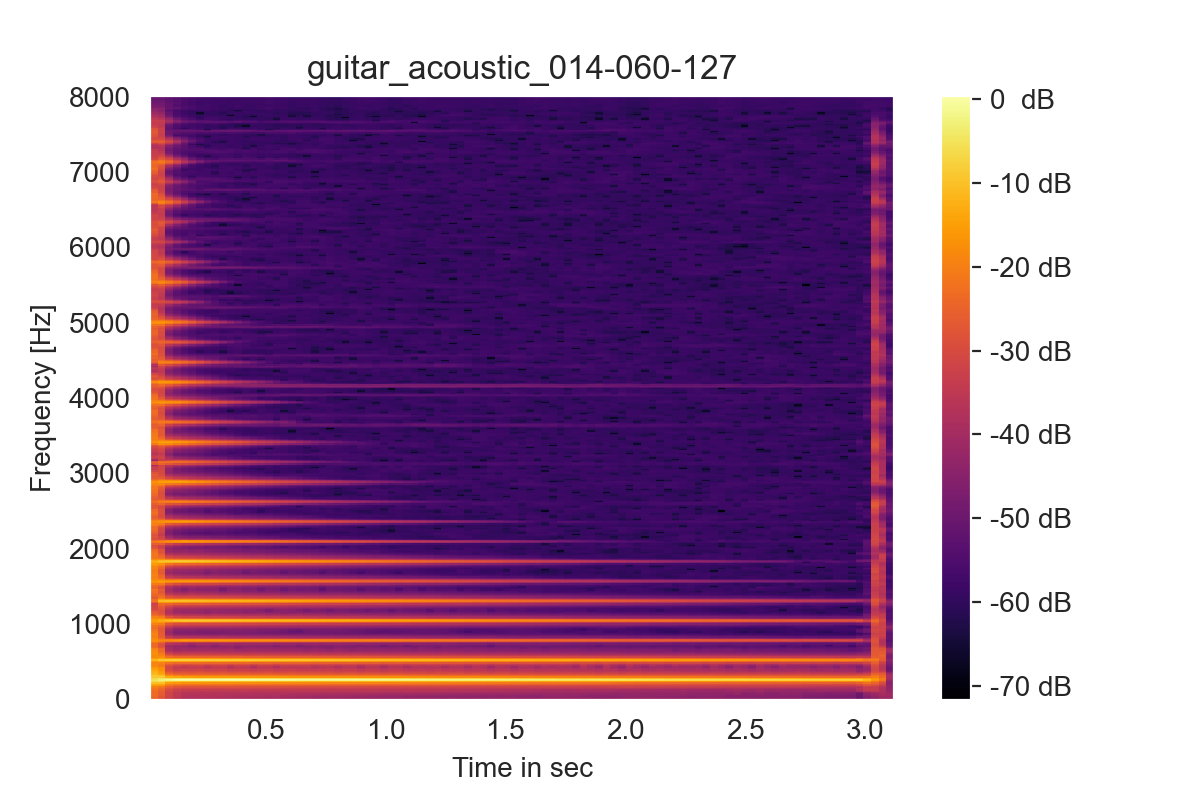
\includegraphics[width=0.55\textwidth]{images/results/single_str/out_guitar_acoustic_014-060-127.png}}&
        \makebox{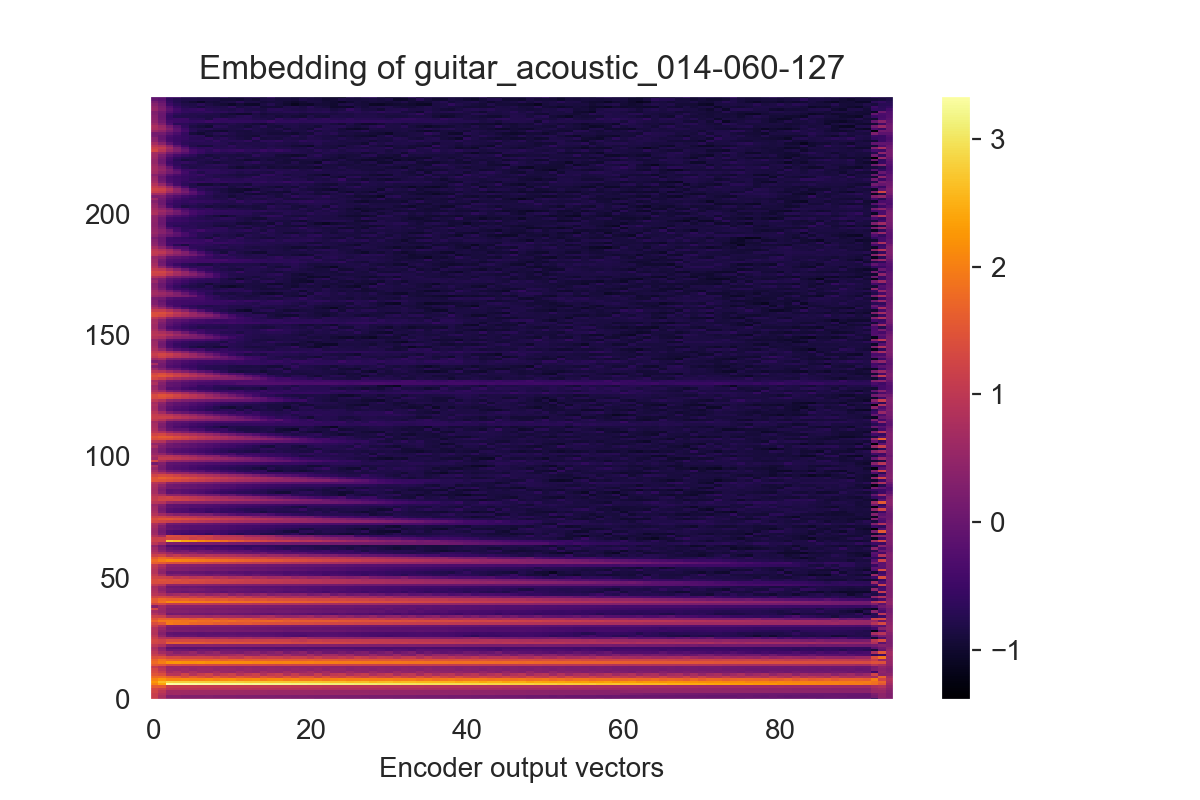
\includegraphics[width=0.55\textwidth]{images/results/single_str/emb_guitar_acoustic_014-060-127.png}}\\
        (a) & (b)
    \end{tabular}}
    \caption{Reconstruction of guitar acoustic ~(a), Embedding of guitar acoustic ~(b)\\single stride model.}
    \label{fig:res_single_str_2D_output_emb}
\end{figure}

With a look on the output of the double-stride network (figure \ref{fig:res_double_str_2D_output_emb}a), it also can be said, that the broad spectra are preserved but with less energy. This can be also noticed when looking on the output spectrogram of the triple stride network (figure \ref{fig:res_triple_str_2D_output_emb}). The latter also shows less energy in the high energy areas and less "precise harmonics" (washed out). 

\begin{figure}[htb!]
    \centering
    \captionsetup{justification=centering}
    \makebox[\textwidth][c]{\begin{tabular}{@{}cc@{}}
        \makebox{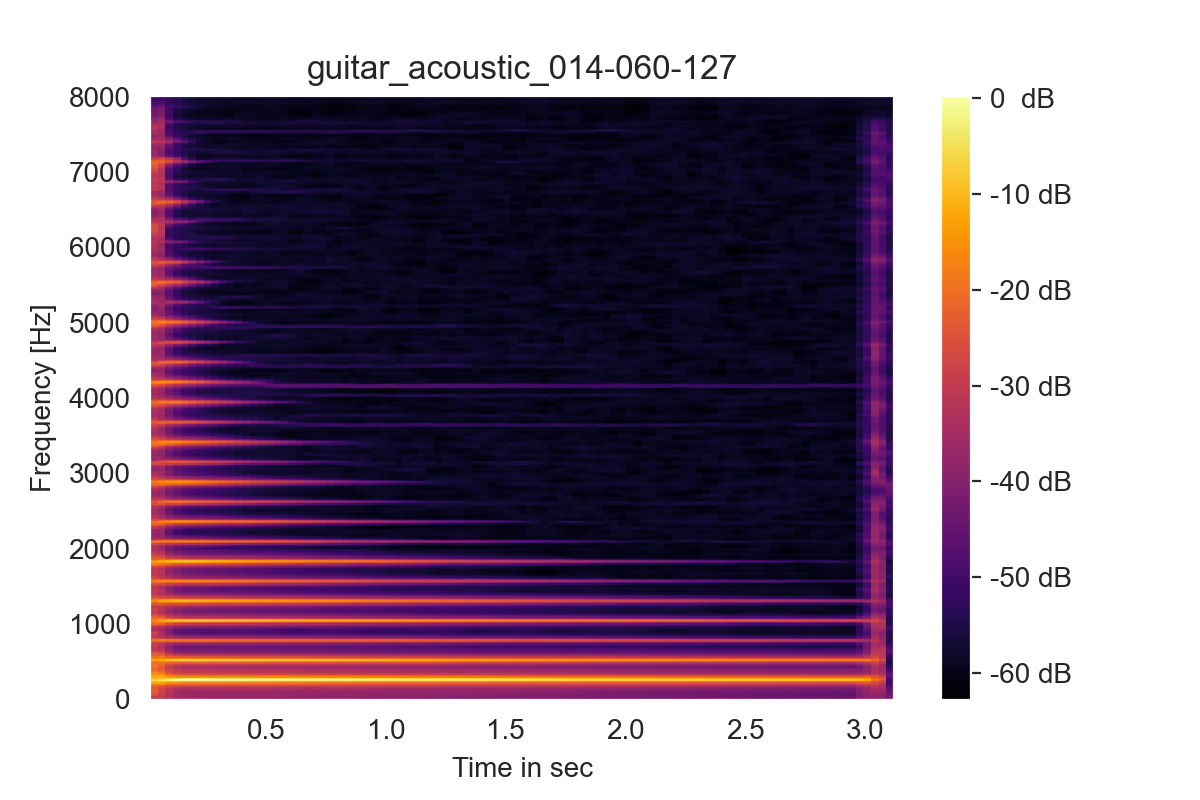
\includegraphics[width=0.55\textwidth]{images/results/double_str/guitar_acoustic_014-060-127.png}}&
        \makebox{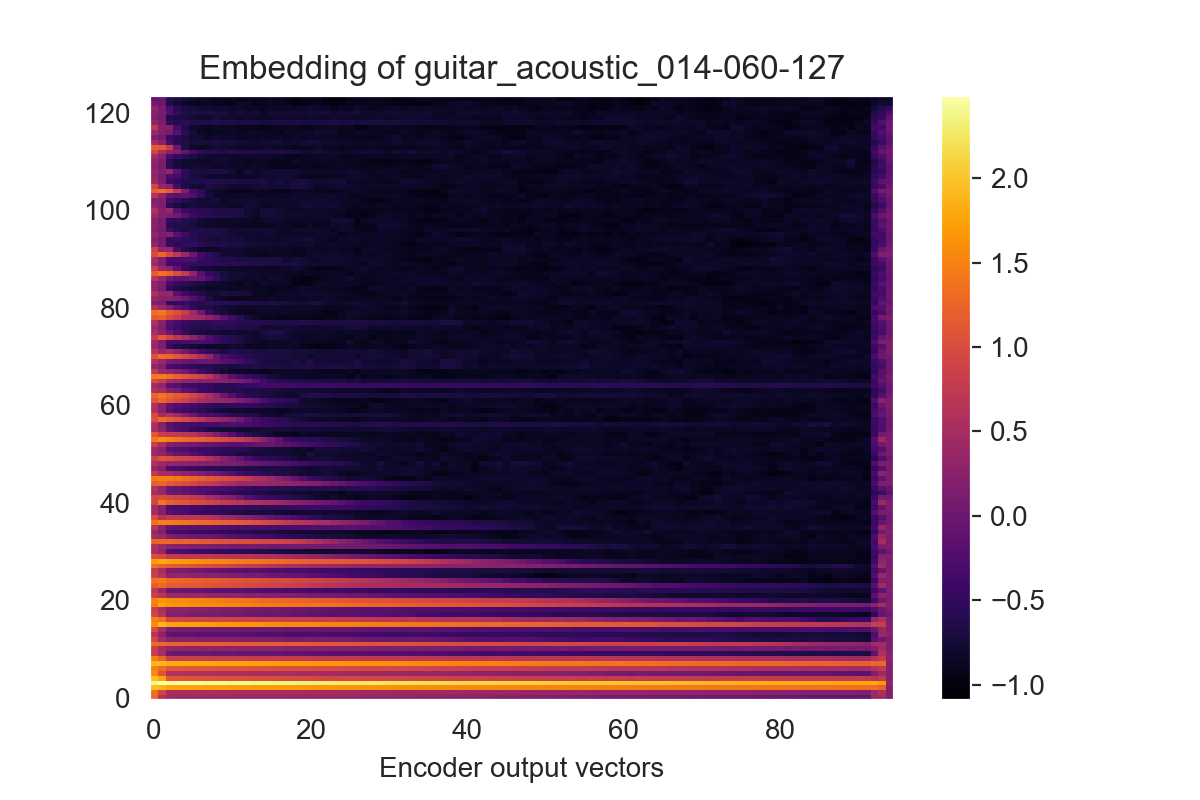
\includegraphics[width=0.55\textwidth]{images/results/double_str/emb_guitar_acoustic_014-060-127.png}}\\
        (a) & (b)
    \end{tabular}}
    \caption{Reconstruction of guitar acoustic ~(a), Embedding of guitar acoustic ~(b)\\double stride model.}
    \label{fig:res_double_str_2D_output_emb}
\end{figure}

Looking onto the embeddings of the two networks it can be said, that those contain signifcantly less values across the y-axis. Comparing it to the input but also the output, despite of the significant compression, the significant harmonic features and general structures are present as positive numbers (regarding the colorscale). As concerning the double strided network, the embedding still has a fine granularity contrary to the one obtained by the triple strided network.

\begin{figure}[htb!]
    \centering
    \captionsetup{justification=centering}
    \makebox[\textwidth][c]{\begin{tabular}{@{}cc@{}}
        \makebox{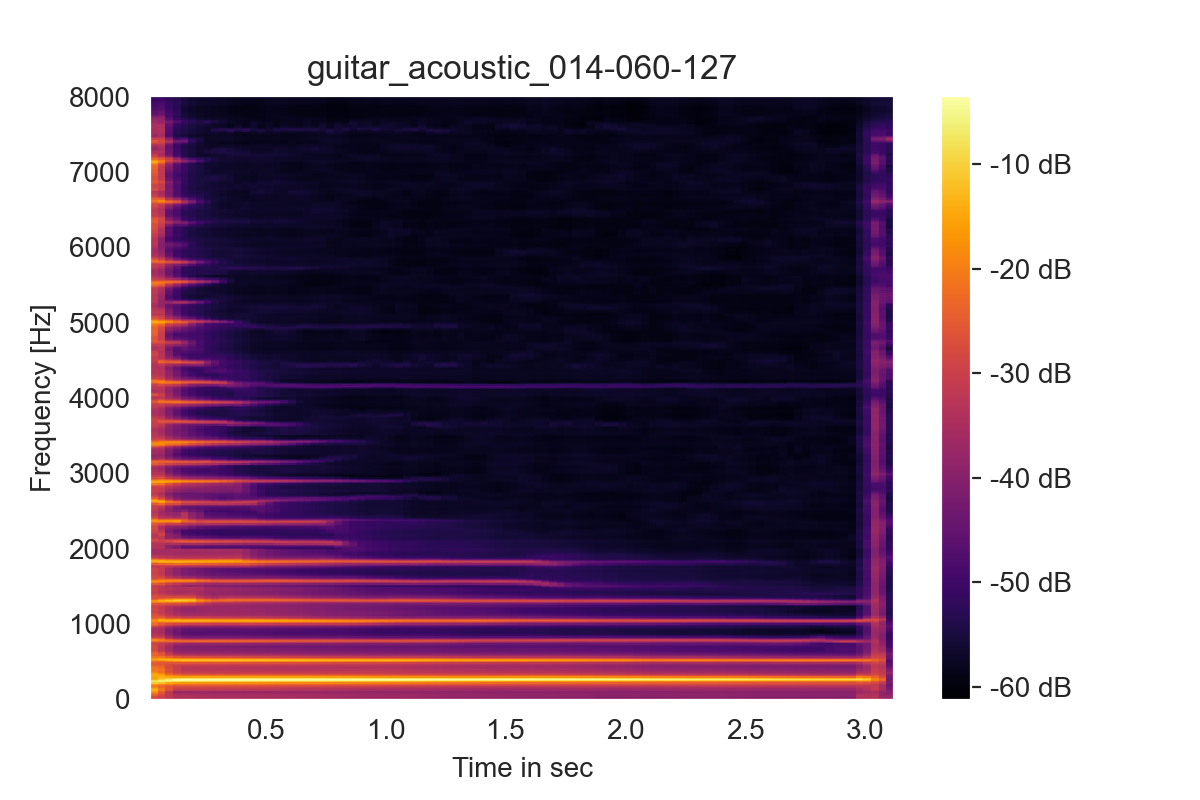
\includegraphics[width=0.55\textwidth]{images/results/triple_str/guitar_acoustic_014-060-127.png}}&
        \makebox{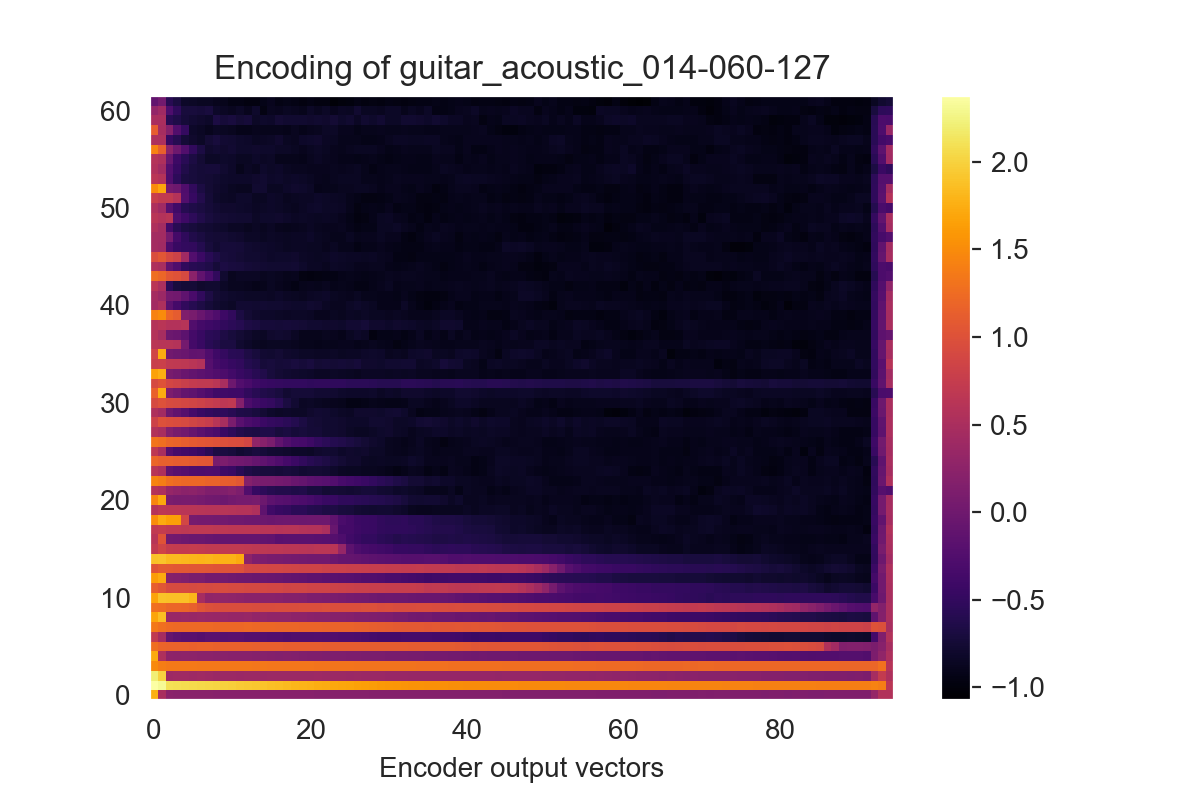
\includegraphics[width=0.55\textwidth]{images/results/triple_str/emb_guitar_acoustic_014-060-127.png}}\\
        (a) & (b)
    \end{tabular}}
    \caption{Reconstruction of guitar acoustic ~(a), Embedding of guitar acoustic ~(b)\\triple stride model.}
    \label{fig:res_triple_str_2D_output_emb}
\end{figure}

\subsection{Experiments with interpolation in embedding}
The results in this section show the resulting outputspectrograms, that got generated by interpolation of the embedding space vectors. This has already been done with the 1D convolutional network where novel sounds could be generated. As with the 2D convolutional networks used in this experiment, promising results in reconstructing single spectrograms could be obtained, this experiments yield interesting results. Not at least, as the embedding got more compressed, this also effects synthesizing new audio, as this is done by interpolating the embeddings. The following graphics (\ref{fig:res_single_str_2D_inter_output}, \ref{fig:res_double_str_2D_inter_output} and \ref{fig:res_tripe} show again the interpolation between the same two instrumental sources, like previously for comparative reasons. Again also the resulting output spectrogram gets displayed to see the final result. The audititory quality again gets assessed and discussed in the next chapter.
When looking at the embeddings in the three graphics, that after interpolating, the features of both instruments are visible in the result. Here it can be seen that the "harmonic" features of the brass sample do not fade contrary to the guitar samples. Nevertheless because of the interpolation the features are present but having lower values as it interpolates mostly between negative and positive numbers. The areas where the both samples have common features (lower harmonics), rather stay equally valued as those have close values. 

\begin{figure}[htb!]
    \centering
    \makebox[\textwidth][c]{\begin{tabular}{@{}cc@{}}
        \makebox{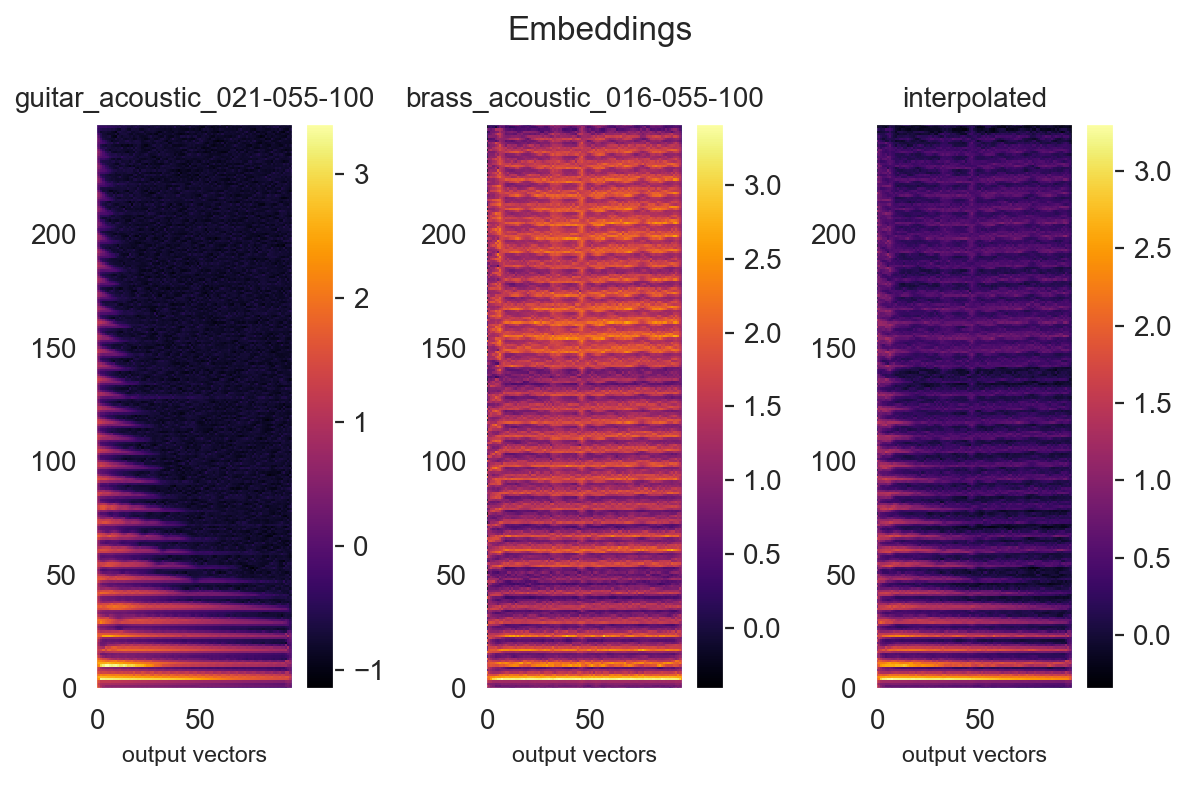
\includegraphics[width=0.55\textwidth]{images/results/single_str/inter_guitar_acoustic_021-055-100&brass_acoustic_016-055-100_original_0.5.png}}&
        \makebox{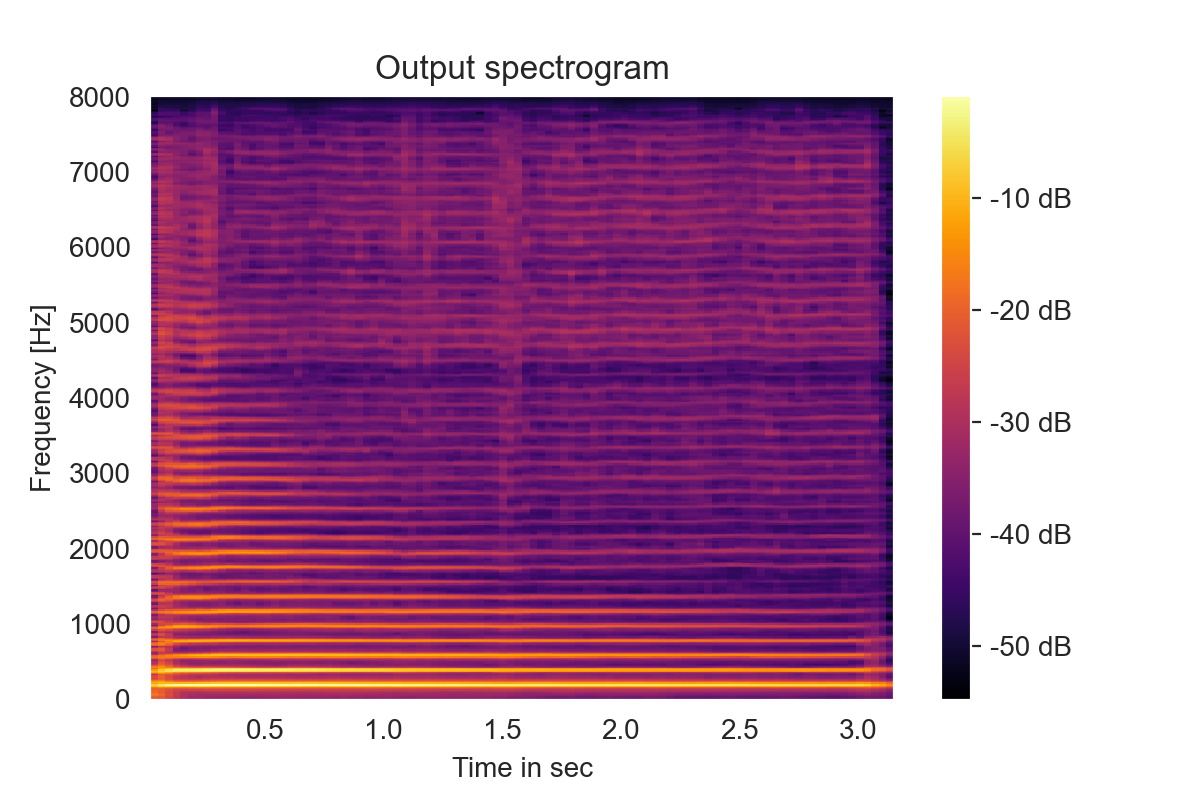
\includegraphics[width=0.55\textwidth]{images/results/single_str/guitar_acoustic_021-055-100&brass_acoustic_016-055-100_output_0.5.png}}\\
        (a) & (b)
    \end{tabular}}
    \caption{embedding interpolation ~(a), output signal ~(b).}
    \label{fig:res_single_str_2D_inter_output}
\end{figure}

By looking again on the decoded output it can be seen, that again both instruments are present. Compared to the result in the first experiments, the guitar sample is more present with these kind of networks. Contrary to the experiment with single sample reconstruction, here the difference between the different strided networks, can be noticed even more. With special notice to the higher harmonics of the original brass samples. Those harmonics appear more precise with the single strided network (see figure \ref{fig:res_single_str_2D_inter_output}b). In the output of the double-stride network in figure \ref{fig:res_double_str_2D_inter_output}b the "contours" coming from the brass sample, are less sharp then with the single stride.

\begin{figure}[htb!]
    \centering
    \makebox[\textwidth][c]{\begin{tabular}{@{}cc@{}}
        \makebox{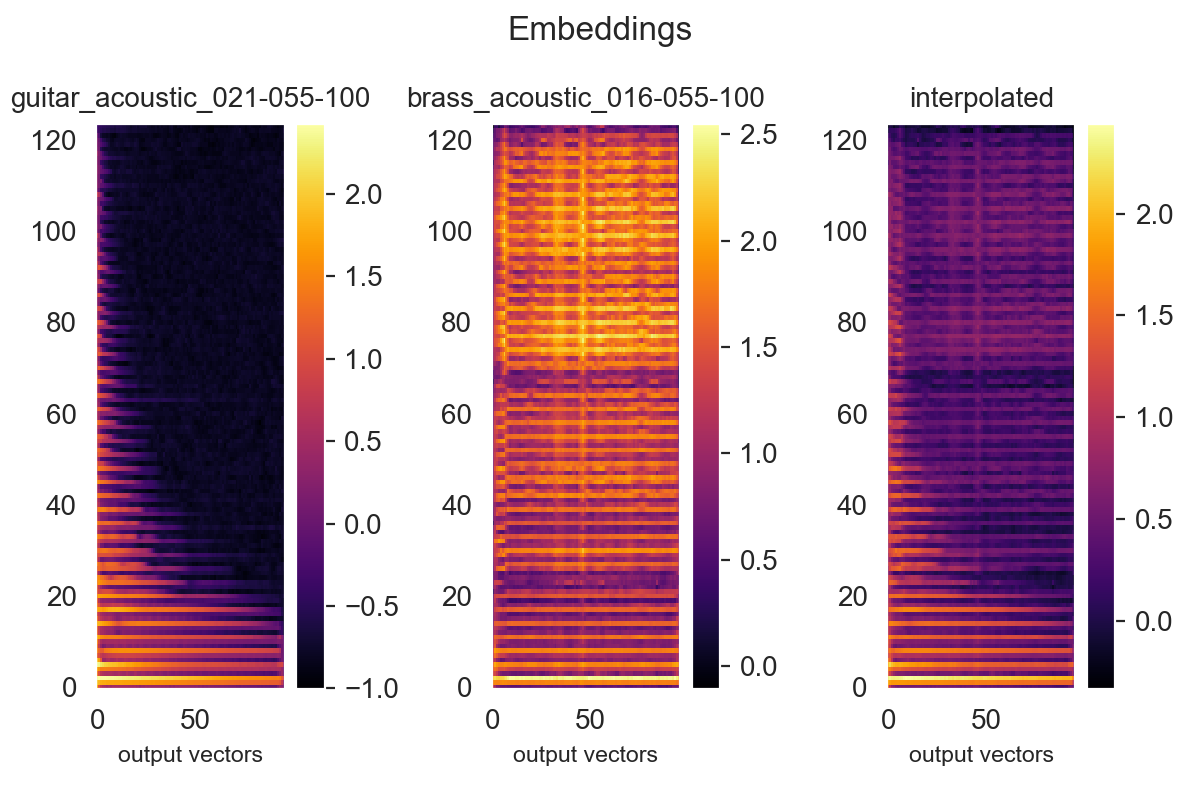
\includegraphics[width=0.55\textwidth]{images/results/double_str/inter_guitar_acoustic_021-055-100&brass_acoustic_016-055-100_original_0.5.png}}&
        \makebox{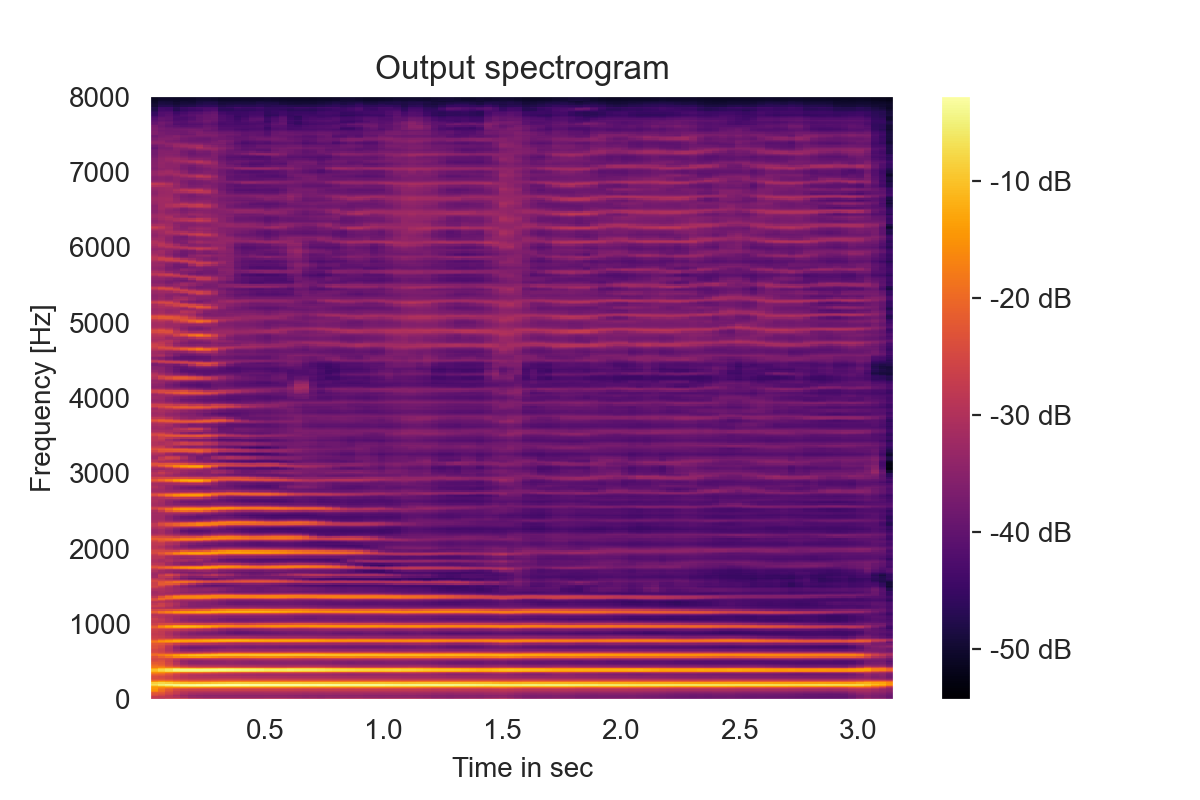
\includegraphics[width=0.55\textwidth]{images/results/double_str/guitar_acoustic_021-055-100&brass_acoustic_016-055-100_output_0.5.png}}\\
        (a) & (b)
    \end{tabular}}
    \caption{embedding interpolation ~(a), output signal ~(b).}
    \label{fig:res_double_str_2D_inter_output}
\end{figure}

Taking the output of the triple strided network (figure \ref{fig:res_triple_str_2D_inter_output}) into account, the difference to the other networks can be seen clearly. The encoded features, again contain the same structure as the input spectrograms, but due to the three-fold striding, just the most significant information is present. Comparing the interpolated embeddings it also can be said that in the latter, the guitar features can be recognized better. Looking at the final output spectrogram in \ref{fig:res_triple_str_2D_inter_output}b it can be seen, that the original fine harmonics aren't present anymore. They are rather washed out. Also the fine changes over time is not as precisely present as with previous network configurations. Nevertheless both instrumental features can be recognized in the final output. 

\begin{figure}[htb!]
    \centering
    \makebox[\textwidth][c]{\begin{tabular}{@{}cc@{}}
        \makebox{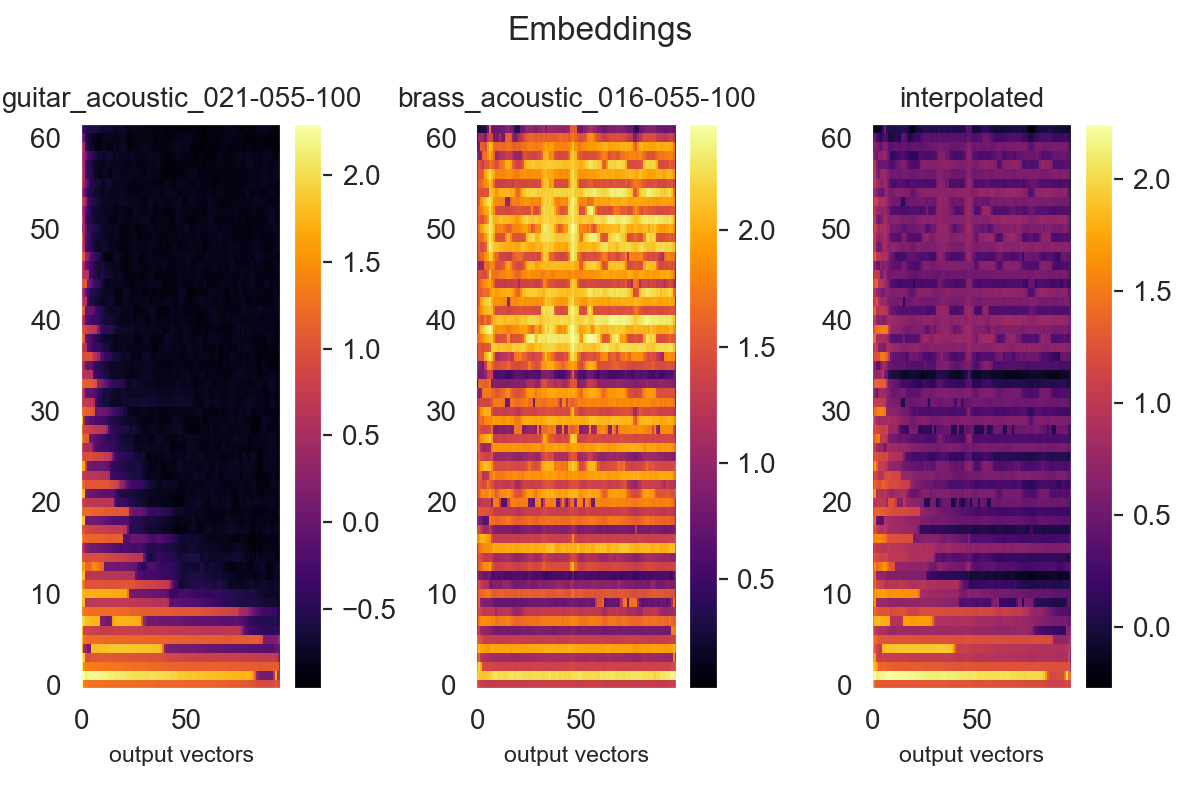
\includegraphics[width=0.55\textwidth]{images/results/triple_str/inter_guitar_acoustic_021-055-100&brass_acoustic_016-055-100_original_0.5.png}}&
        \makebox{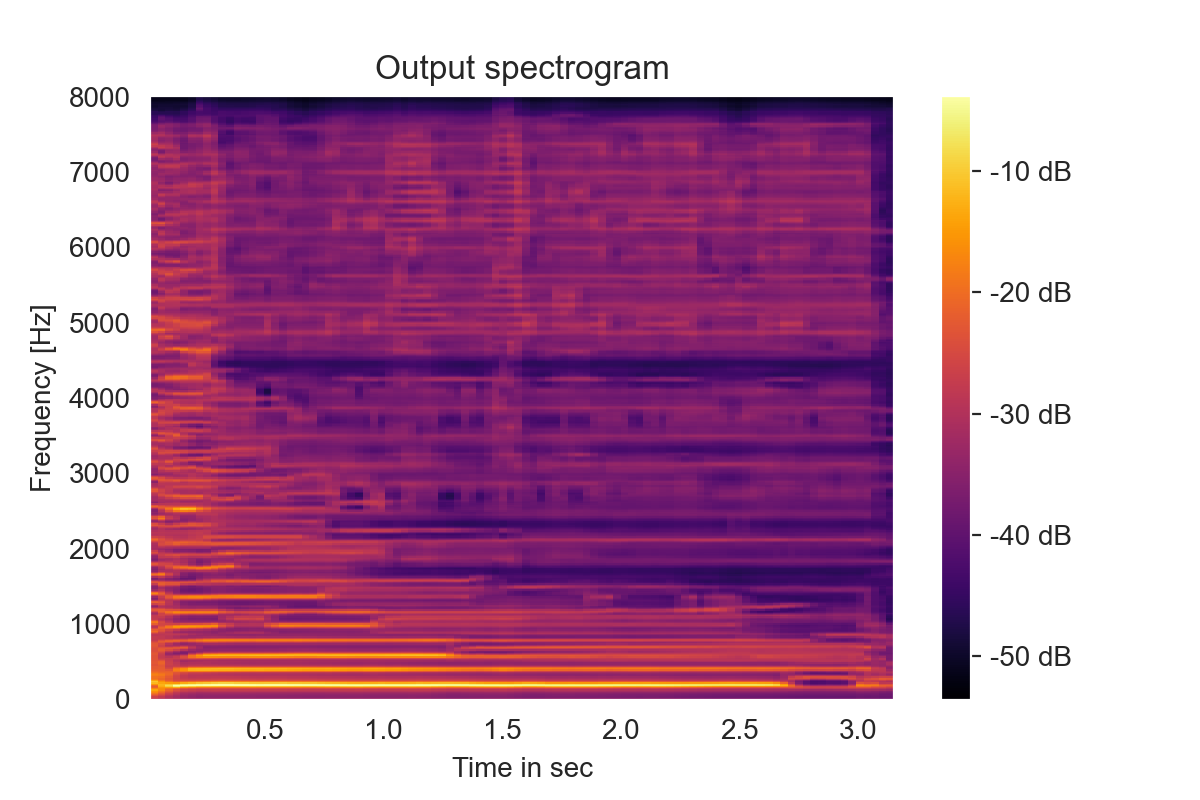
\includegraphics[width=0.55\textwidth]{images/results/triple_str/guitar_acoustic_021-055-100&brass_acoustic_016-055-100_output_0.5.png}}\\
        (a) & (b)
    \end{tabular}}
    \caption{embedding interpolation ~(a), output signal ~(b)}
    \label{fig:res_triple_str_2D_inter_output}
\end{figure}

Again in the discussion part, the auditive quality of all outputs presented here, with and without energy correction, gets assessed and brought into relation with the here displayed spectrograms.

\section{Results with mel-spectrograms}

The final experiments are again done with a 2D convolutional network, but using mel-scale instead of log-magnitude. In chapter \ref{cha:Experiment} under section \ref{sec:exp_mel} an introduction to the mel-scale has been given, as experiments were done using this scale. As this scale is a compressed version of the log-magnitude scale and emphasizes the lower frequencies, these experiments are expected to bring different but interesting results. This is again meant regarding the model performance but also towards the quality of reconstructing spectrograms with or without modification of the embeddings. The results again get depicted in tables filled with the MSE scores of training, validation and testing but also the scores regarding specific pitch classes of the test set. Later on again graphics containing the output spectrograms and embeddings with and without interpolation. Again three different networks with single, double and triple striding were used. Those are similar in their structure to the ones used with log-magnitude spectrograms, which was already explained in the previous chapter.

The following table \ref{tab:res_scores_2D_mel} shows the training, validation and testing scores of all three different networks. First of all the MSE scores of all networks are significantly, higher than the ones of the log-magnitude networks. An exception makes the testing score of the single-stride network as it is equally to the training score of the triple-strided log-magnitude network. The scores between the networks, also increase with the amount of compression, making the single-stride network again the best performing network regarding its score. Interestingly the validation score of the single-stride network, is the only one that is higher as its corresponding training score. The double- and triple-stride networks therefore show that they have a lower score on reconstructing unseen data. Again the auditory quality will get assessed in the next chapter \ref{cha:Discussion}.

\begin{table}[htb!]
    \centering
    \begin{tabular}{|c|c|c|c|}
        \hline
         & \textbf{single-stride} & \textbf{double-stride} & \textbf{triple-stride} \\
         \hline
        \textbf{Training} & 30,579 & 49,685 & 62,833 \\
        \hline
        \textbf{Validation} & 31,084 & 48,439 & 60,471\\
        \hline
        \textbf{Test} & 18,322 & 33,689 & 43,300\\
        \hline
    \end{tabular}
    \caption{MSE-Scores 2D convolutional autoencoder - mel-scale - single stride (15 epochs), double stride (21 epochs), triple stride (68 epochs)}
    \label{tab:res_scores_2D_mel}
\end{table}

\begin{table}[htb!]
\centering
\begin{tabular}{|c|c|c|c|}
\hline
\textbf{pitch} & \textbf{single-stride} & \textbf{double-stride} & \textbf{triple-stride} \\ \hline
\textbf{030}   & 17,178                 & 24,567                 & 30,302                 \\ \hline
\textbf{035}   & 18,380                 & 26,142                 & 36,509                 \\ \hline
\textbf{040}   & 19,382                 & 34,125                 & 44,062                 \\ \hline
\textbf{045}   & 22,036                 & 55,770                 & 51,097                 \\ \hline
\textbf{050}   & 22,398                 & 41,101                 & 49,810                 \\ \hline
\textbf{055}   & 22,159                 & 43,215                 & 56,664                 \\ \hline
\textbf{060}   & 21,472                 & 40,493                 & 54,690                 \\ \hline
\textbf{065}   & 22,303                 & 40,140                 & 51,926                 \\ \hline
\textbf{070}   & 23,875                 & 41,950                 & 50,904                 \\ \hline
\textbf{075}   & 24,571                 & 37,424                 & 49,297                 \\ \hline
\textbf{080}   & 29,053                 & 43,572                 & 60,926                 \\ \hline
\textbf{085}   & 29,395                 & 46,822                 & 62,750                 \\ \hline
\textbf{090}   & 33,316                 & 51,408                 & 72,206                 \\ \hline
\textbf{095}   & 31,385                 & 51,593                 & 70,607                 \\ \hline
\textbf{100}   & 32,129                 & 51,426                 & 70,890                 \\ \hline
\end{tabular}
\caption{MSE-Scores for specific pitch classes using 2D convolutional autoencoder using mel-scale.}
\label{tab:res_scores_2D_pitch_mel}
\end{table}

\subsection{Experiments of single reconstruction}

\begin{figure}[htb!]
    \centering
    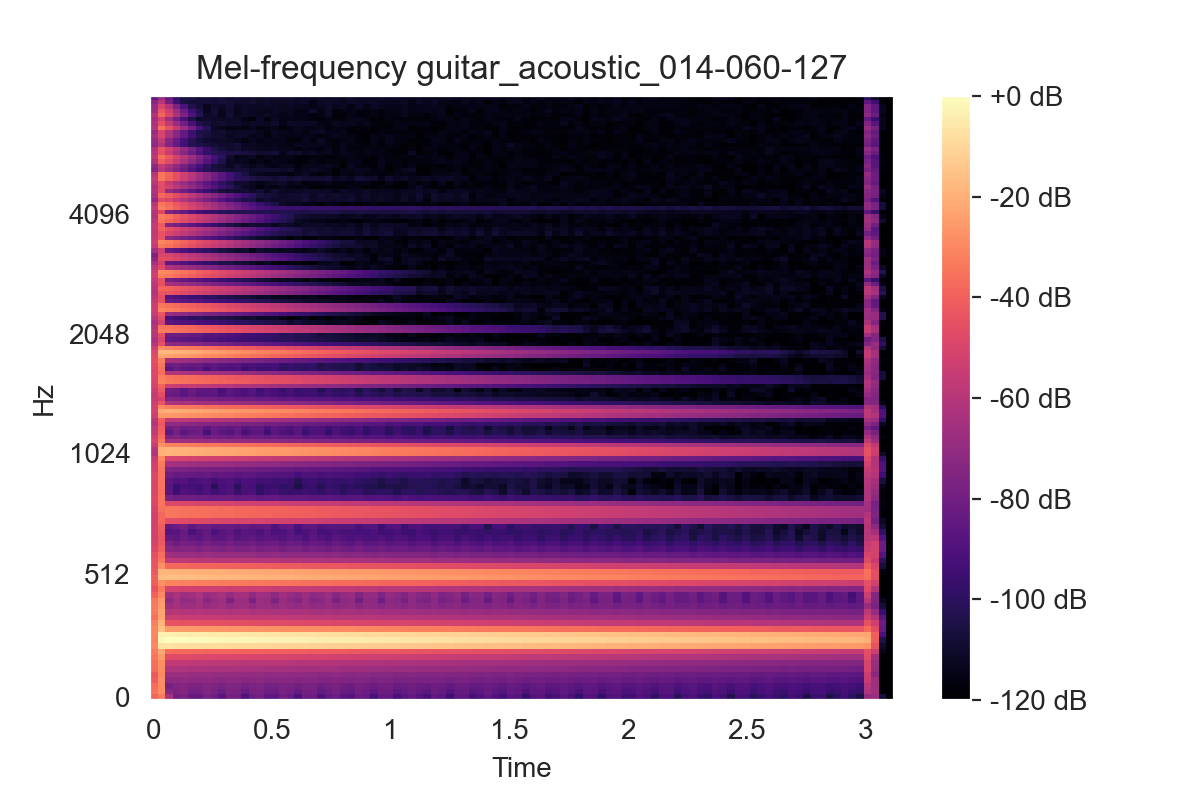
\includegraphics[width=0.5\textwidth]{images/results/mel_guitar_acoustic_014-060-127.png}
    \caption{original mel-spectrogram of guitar acoustic.}
    \label{fig:res_2D_mel_guit}
\end{figure}

\begin{figure}[htb!]
    \centering
    \captionsetup{justification=centering}
    \makebox[\textwidth][c]{\begin{tabular}{@{}cc@{}}
        \makebox{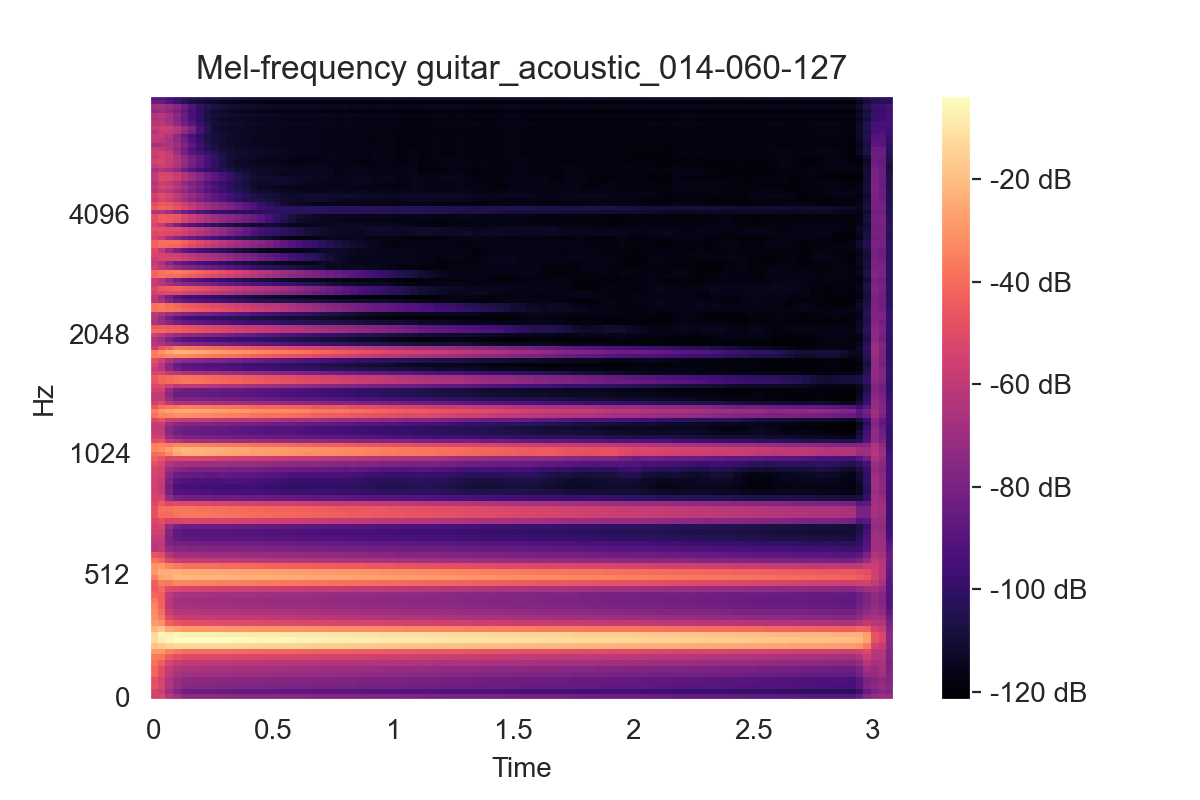
\includegraphics[width=0.55\textwidth]{images/results/mel_single_str/guitar_acoustic_014-060-127.png}}&
        \makebox{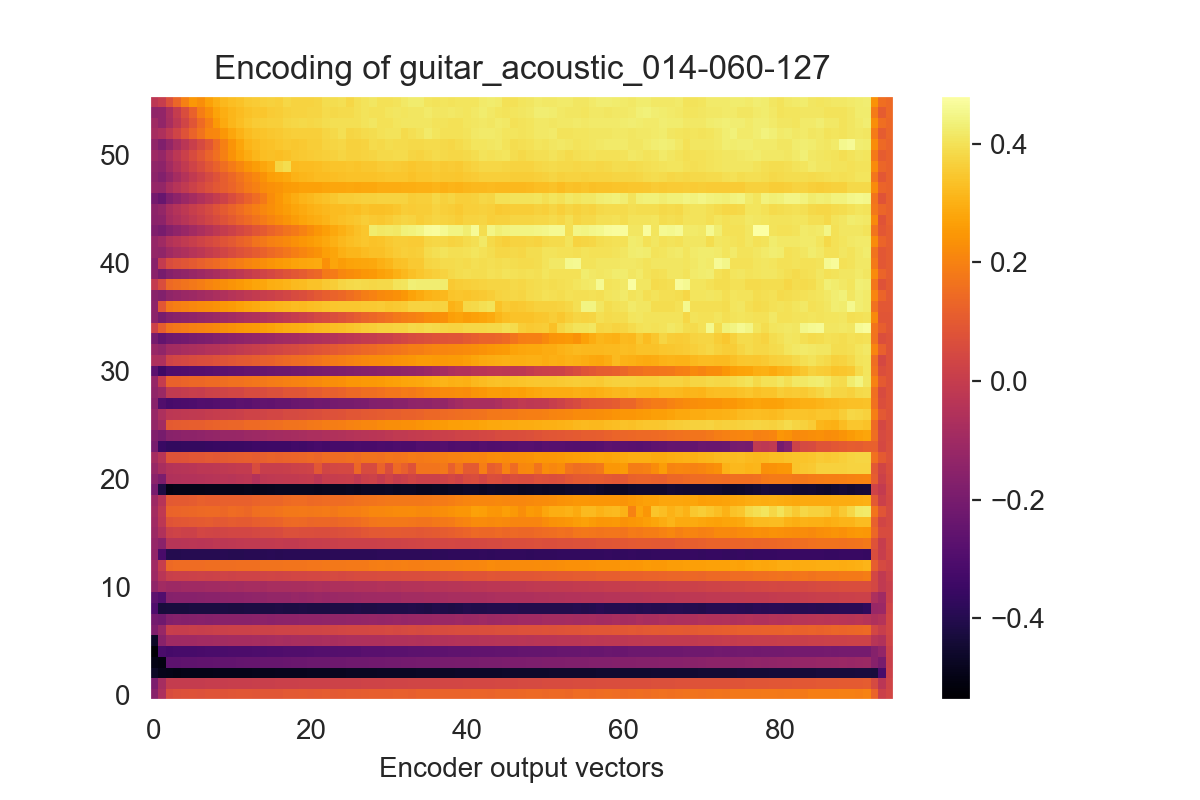
\includegraphics[width=0.55\textwidth]{images/results/mel_single_str/emb_guitar_acoustic_014-060-127.png}}\\
        (a) & (b)
    \end{tabular}}
    \caption{Reconstruction of guitar acoustic ~(a), Embedding of guitar acoustic ~(b)\\single stride model.}
    \label{fig:res_mel_single_str_2D_output_emb}
\end{figure}



\begin{figure}[htb!]
    \centering
    \captionsetup{justification=centering}
    \makebox[\textwidth][c]{\begin{tabular}{@{}cc@{}}
        \makebox{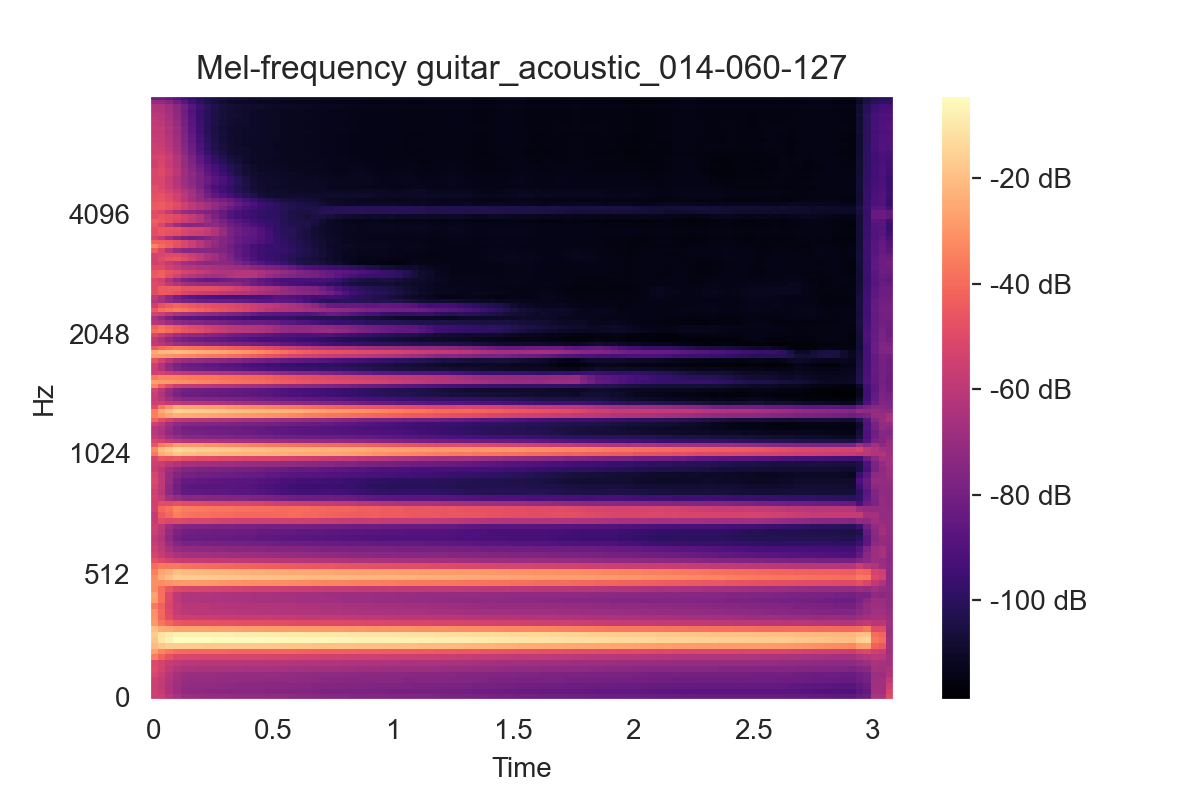
\includegraphics[width=0.55\textwidth]{images/results/mel_double_str/guitar_acoustic_014-060-127.png}}&
        \makebox{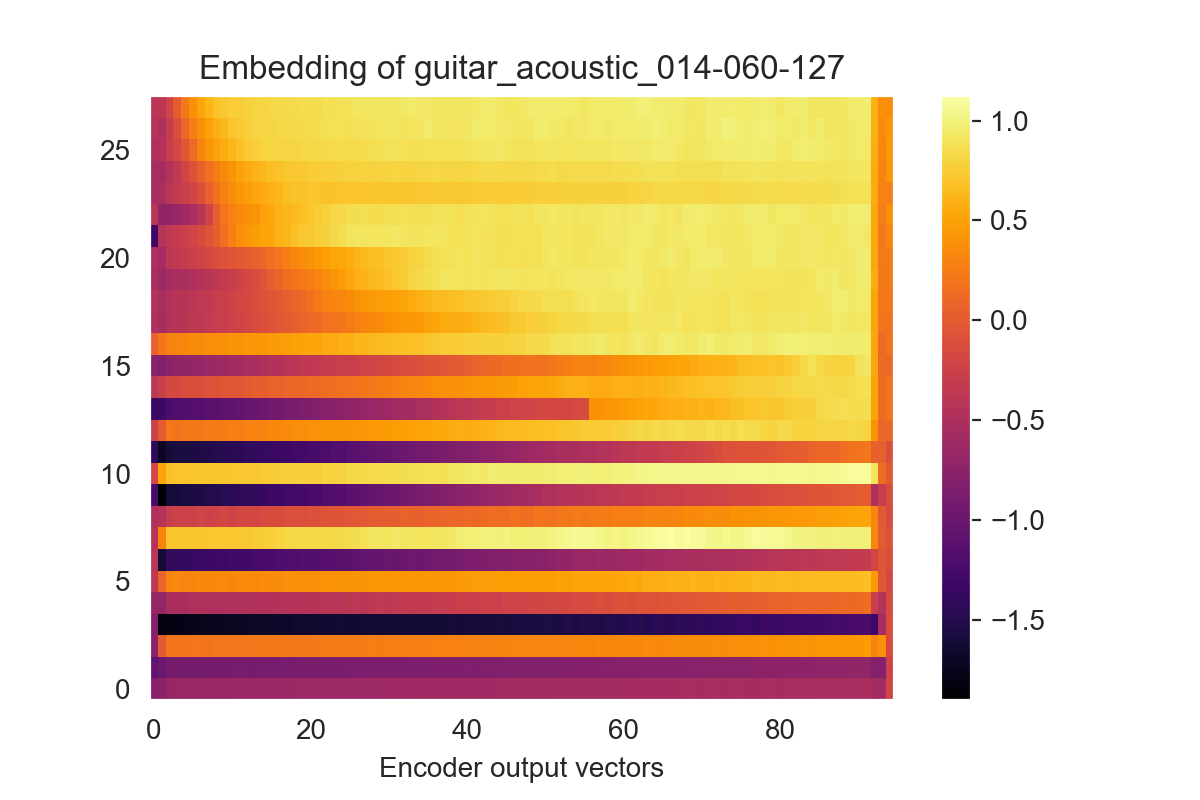
\includegraphics[width=0.55\textwidth]{images/results/mel_double_str/emb_guitar_acoustic_014-060-127.png}}\\
        (a) & (b)
    \end{tabular}}
    \caption{Reconstruction of guitar acoustic ~(a), Embedding of guitar acoustic ~(b)\\double stride model.}
    \label{fig:res_mel_double_str_2D_output_emb}
\end{figure}

\begin{figure}[htb!]
    \centering
    \captionsetup{justification=centering}
    \makebox[\textwidth][c]{\begin{tabular}{@{}cc@{}}
        \makebox{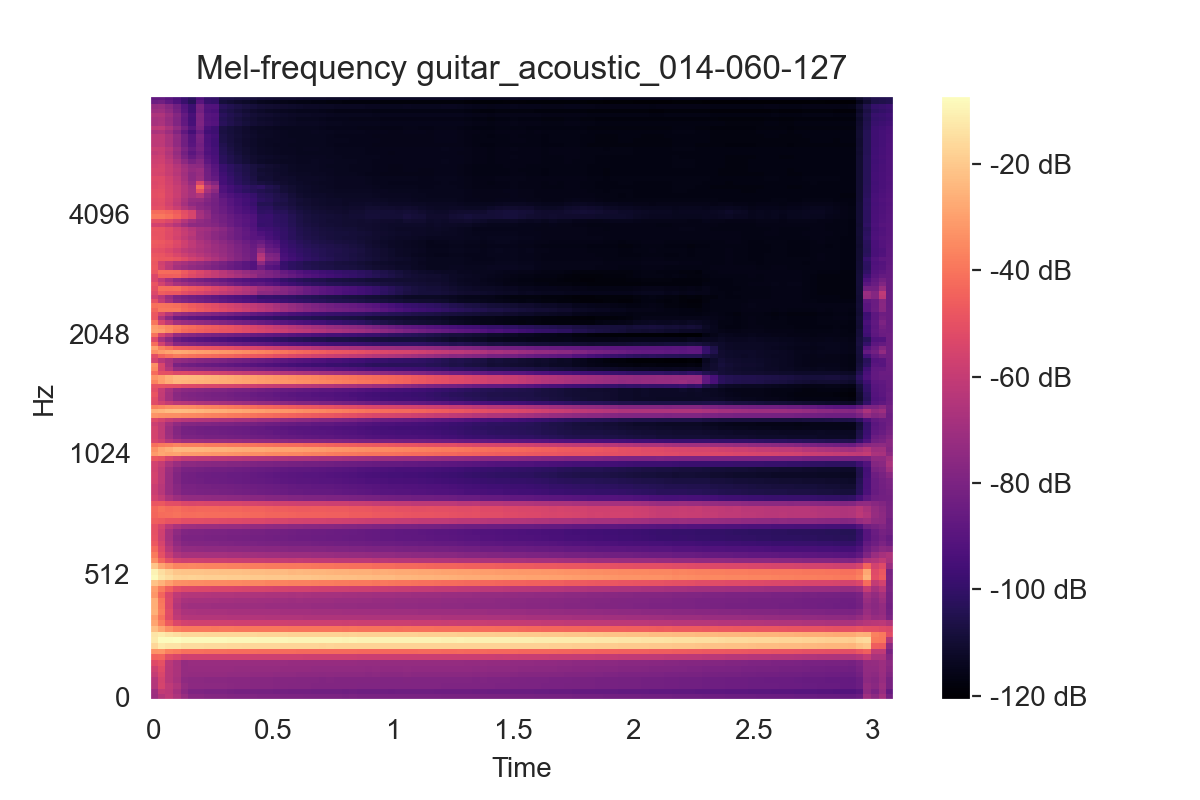
\includegraphics[width=0.55\textwidth]{images/results/mel_triple_str/guitar_acoustic_014-060-127.png}}&
        \makebox{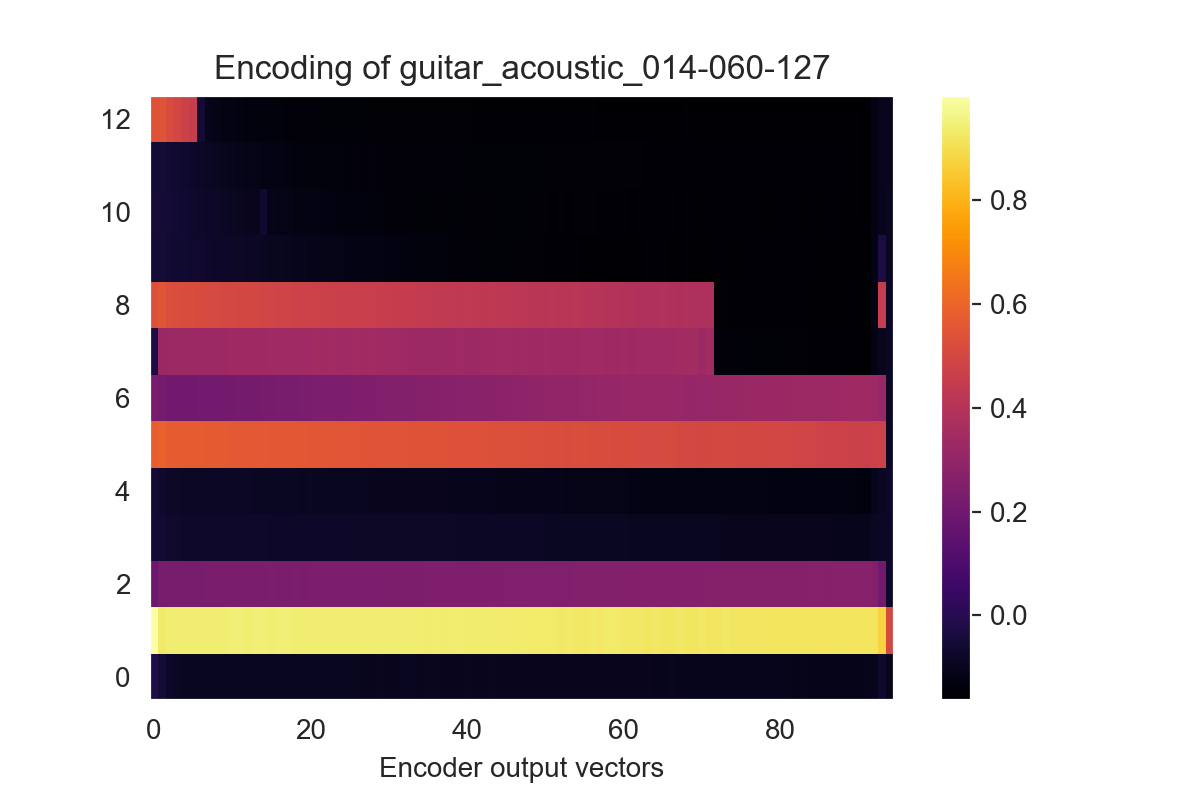
\includegraphics[width=0.55\textwidth]{images/results/mel_triple_str/emb_guitar_acoustic_014-060-127.png}}\\
        (a) & (b)
    \end{tabular}}
    \caption{Reconstruction of guitar acoustic ~(a), Embedding of guitar acoustic ~(b)\\triple stride model.}
    \label{fig:res_mel_triple_str_2D_output_emb}
\end{figure}

\subsection{Experiments with interpolation in embedding}

\begin{figure}[htb!]
    \centering
    \captionsetup{justification=centering}
    \makebox[\textwidth][c]{\begin{tabular}{@{}cc@{}}
        \makebox{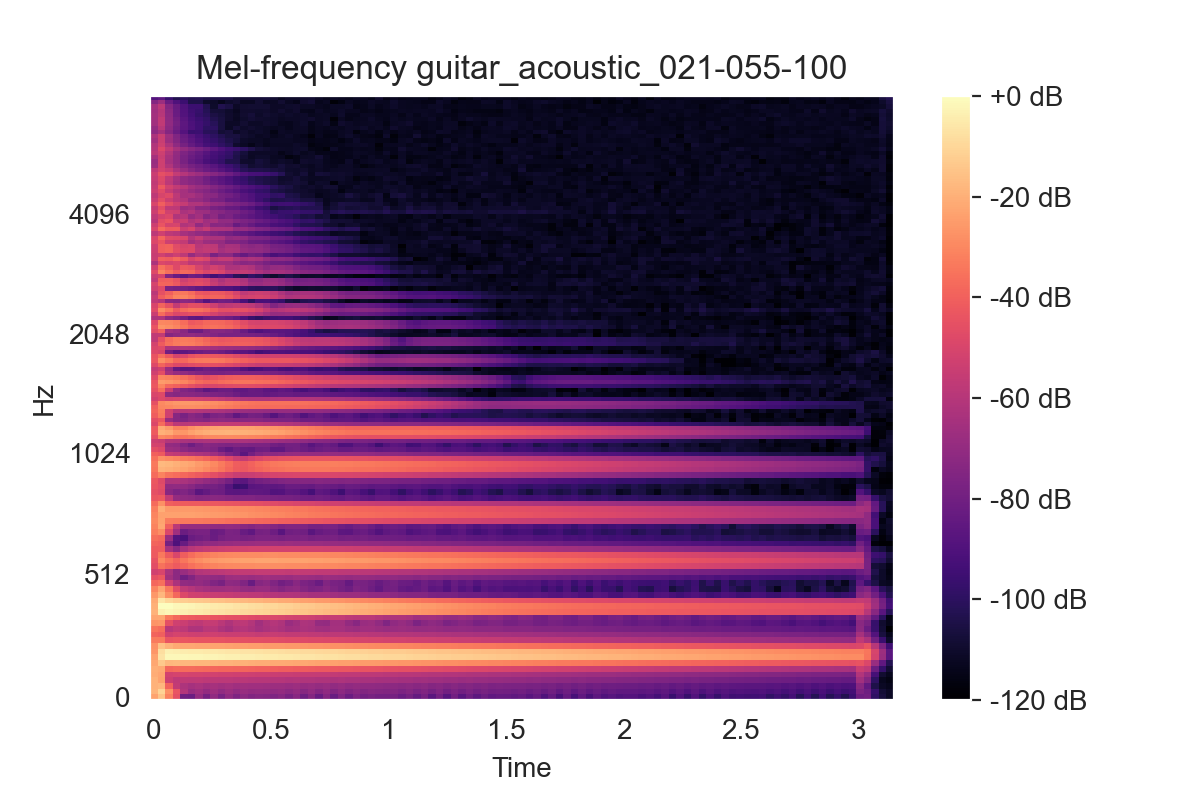
\includegraphics[width=0.55\textwidth]{images/results/mel_guitar_acoustic_021-055-100.png}}&
        \makebox{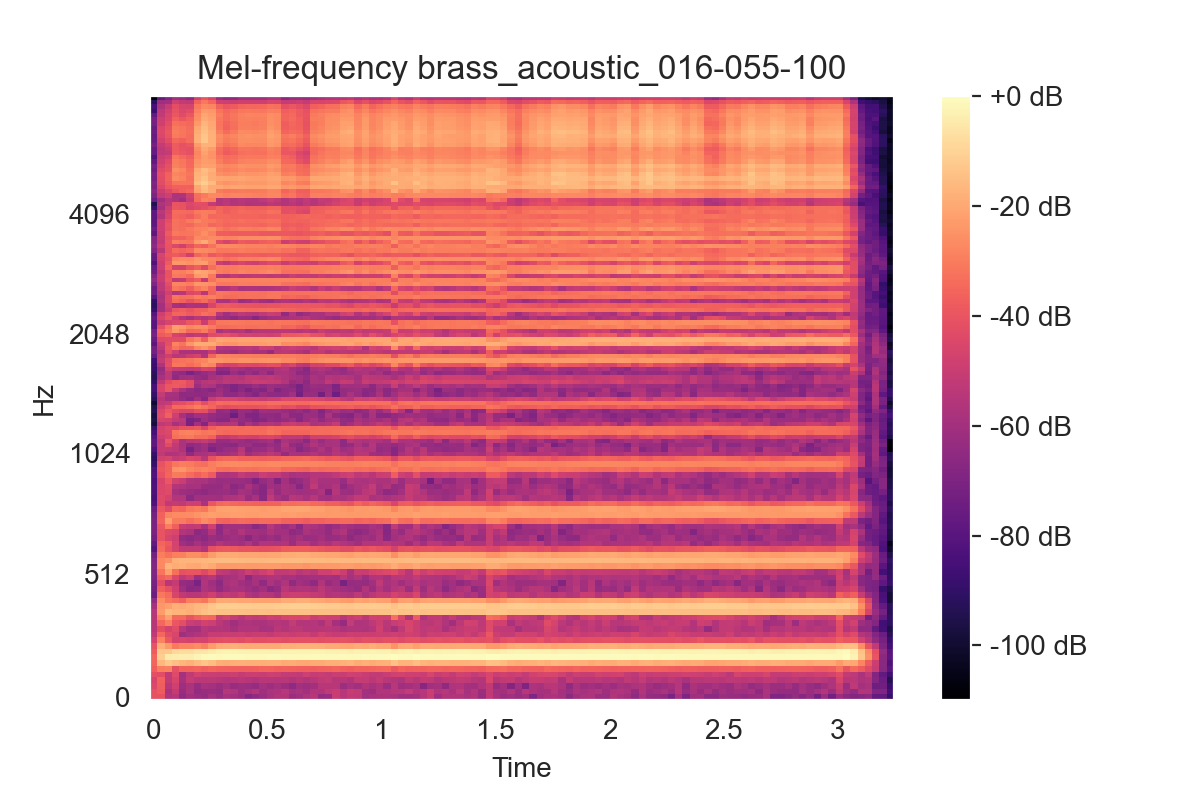
\includegraphics[width=0.55\textwidth]{images/results/mel_brass_acoustic_016-055-100.png}}\\
        (a) & (b)
    \end{tabular}}
    \caption{original guitar acoustic ~(a), original brass acoustic
    ~(b)}
    \label{fig:res_mel_original_guit_brass}
\end{figure}

\begin{figure}[htb!]
    \centering
    \makebox[\textwidth][c]{\begin{tabular}{@{}cc@{}}
        \makebox{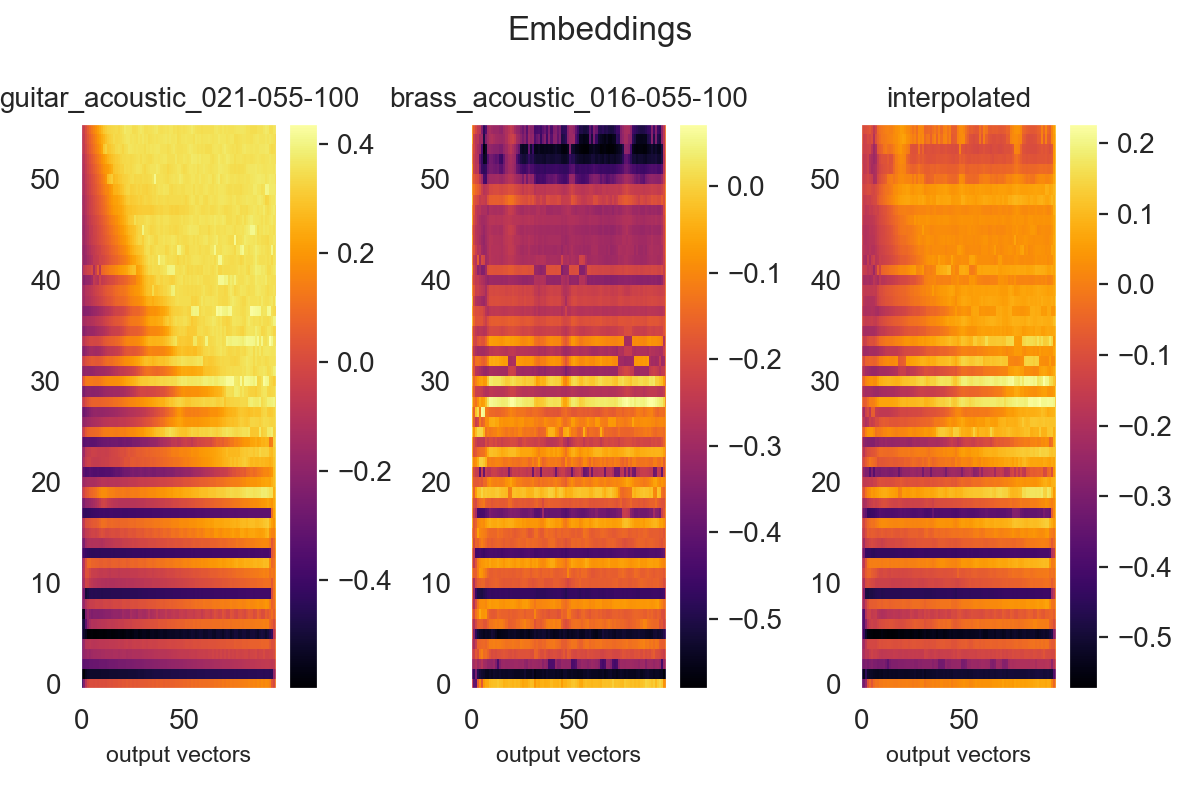
\includegraphics[width=0.55\textwidth]{images/results/mel_single_str/inter_guitar_acoustic_021-055-100&brass_acoustic_016-055-100_original_0.5.png}}&
        \makebox{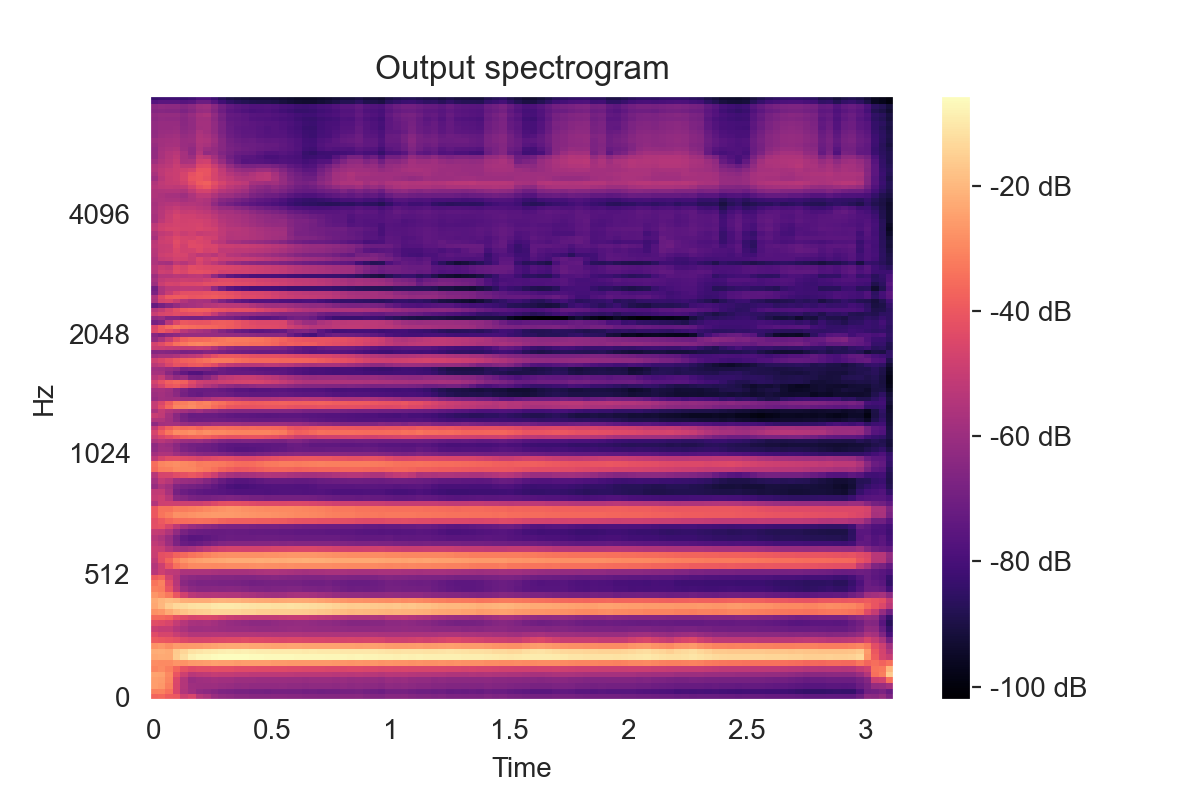
\includegraphics[width=0.55\textwidth]{images/results/mel_single_str/guitar_acoustic_021-055-100&brass_acoustic_016-055-100_output_0.5.png}}\\
        (a) & (b)
    \end{tabular}}
    \caption{embedding interpolation ~(a), output signal ~(b).}
    \label{fig:res_mel_single_str_2D_inter_output}
\end{figure}

\begin{figure}[htb!]
    \centering
    \makebox[\textwidth][c]{\begin{tabular}{@{}cc@{}}
        \makebox{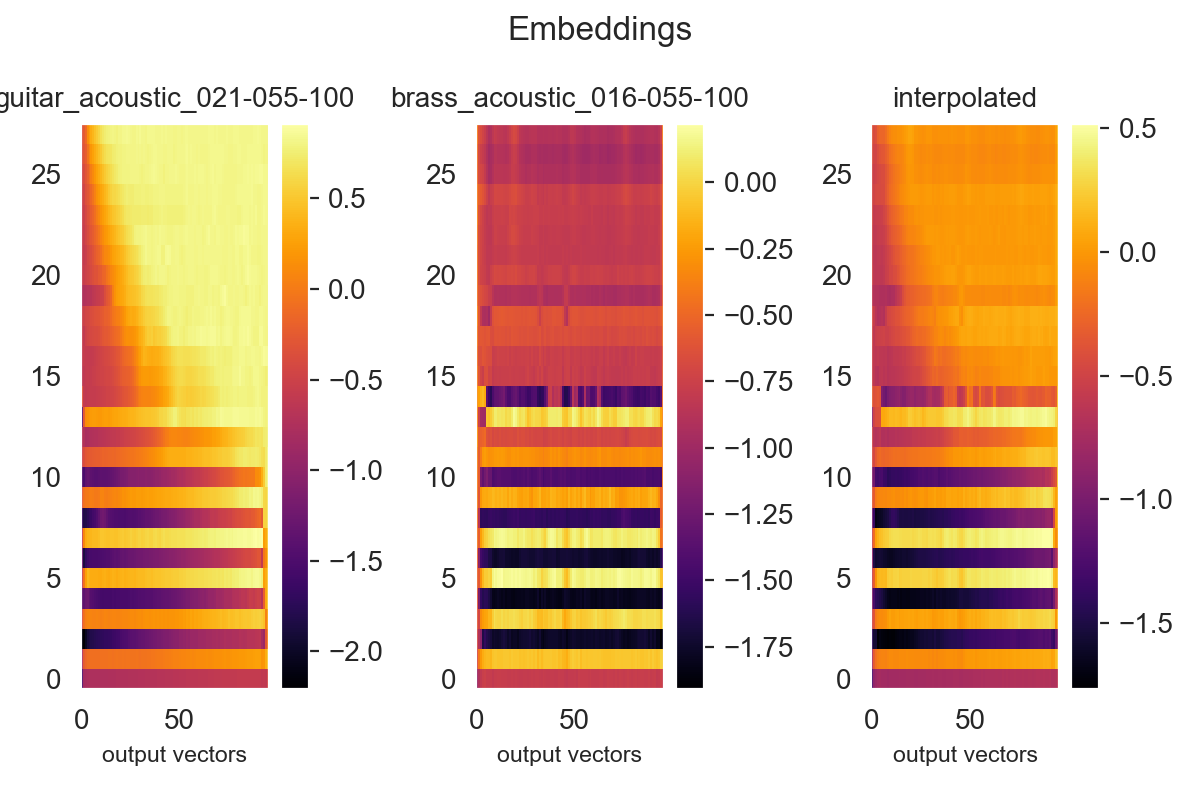
\includegraphics[width=0.55\textwidth]{images/results/mel_double_str/inter_guitar_acoustic_021-055-100&brass_acoustic_016-055-100_original_0.5.png}}&
        \makebox{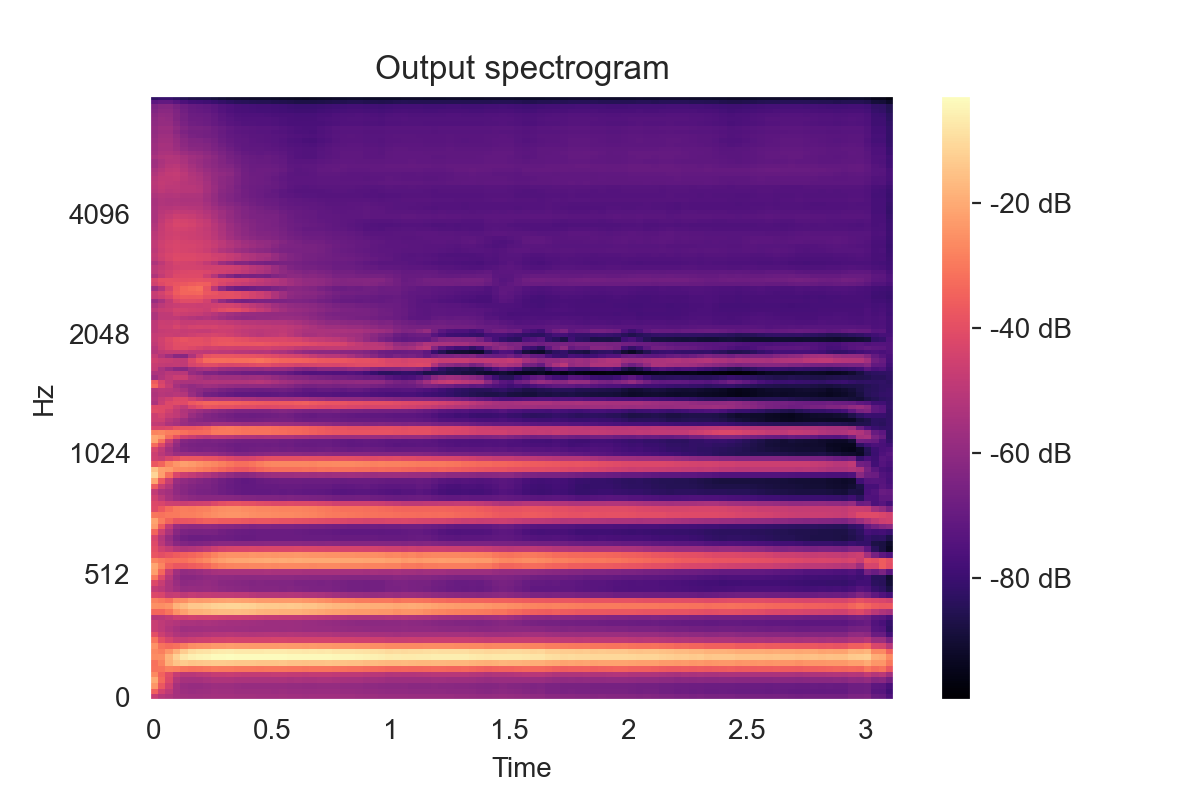
\includegraphics[width=0.55\textwidth]{images/results/mel_double_str/guitar_acoustic_021-055-100&brass_acoustic_016-055-100_output_0.5.png}}\\
        (a) & (b)
    \end{tabular}}
    \caption{embedding interpolation ~(a), output signal ~(b).}
    \label{fig:res_mel_double_str_2D_inter_output}
\end{figure}

\begin{figure}[htb!]
    \centering
    \makebox[\textwidth][c]{\begin{tabular}{@{}cc@{}}
        \makebox{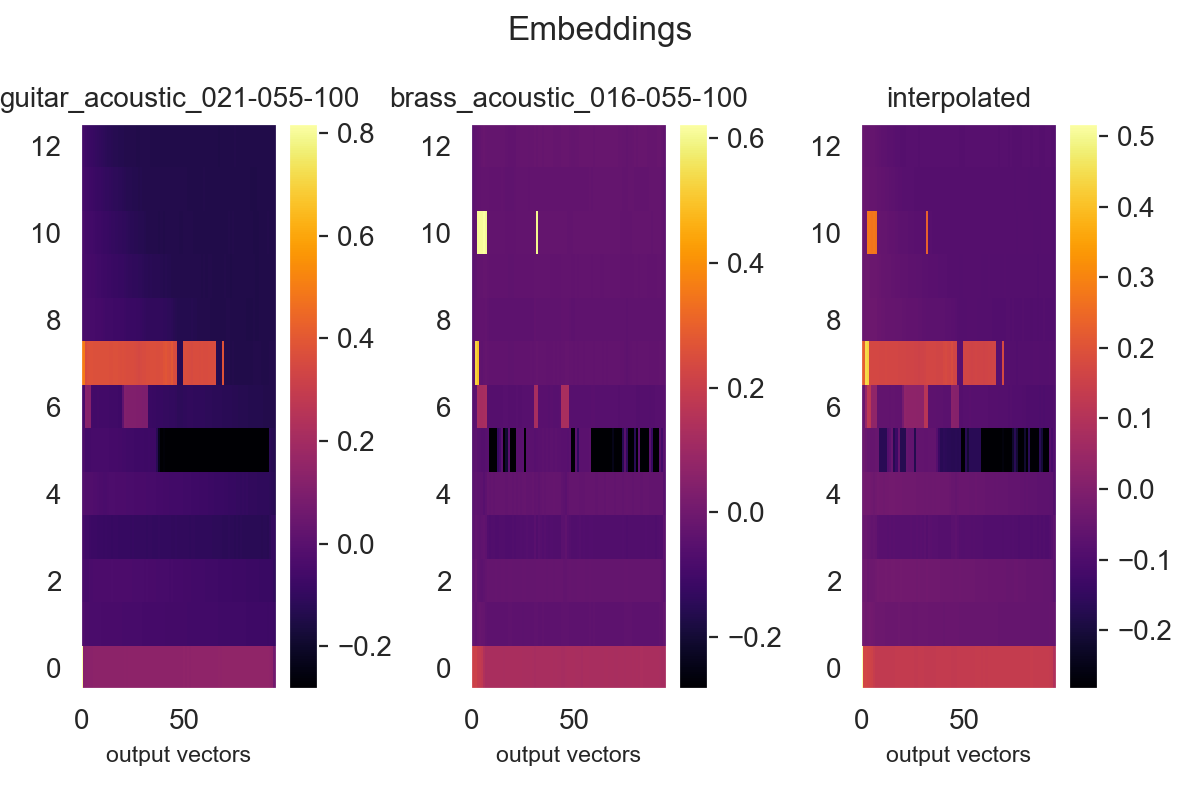
\includegraphics[width=0.55\textwidth]{images/results/mel_triple_str/inter_guitar_acoustic_021-055-100&brass_acoustic_016-055-100_original_0.5.png}}&
        \makebox{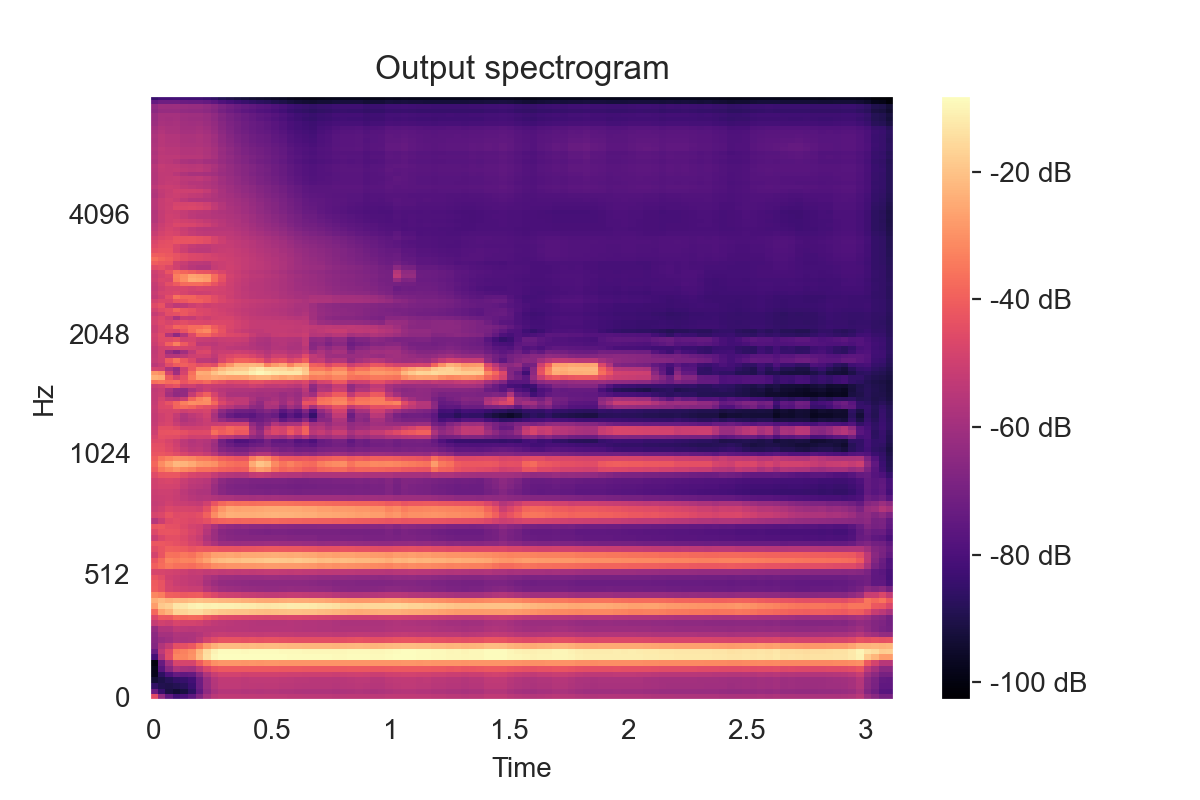
\includegraphics[width=0.55\textwidth]{images/results/mel_triple_str/guitar_acoustic_021-055-100&brass_acoustic_016-055-100_output_0.5.png}}\\
        (a) & (b)
    \end{tabular}}
    \caption{embedding interpolation ~(a), output signal ~(b).}
    \label{fig:res_mel_triple_str_2D_inter_output}
\end{figure}